% !TeX program = xelatex
% 2026 全国大学生数学建模竞赛论文骨架（电子版）
% 提交前请删除所有“待填写”提示，并核对 paper/README.md 中的清单。

\documentclass[withoutpreface,bwprint]{cumcmthesis}
\usepackage{cumcm2026}

\title{无线电干扰源的快速自动定位与清除（草稿）}

\begin{document}

\maketitle

\begin{abstract}
本文研究半径为 $1800\ \mathrm m$ 的圆形区域内无线电干扰源的自动定位与清除问题。示向误差、接收距离和发射方向都存在不确定性，我们建立了从\textbf{几何交会}、\textbf{选点规划}到\textbf{多源搜索清除}的递进式模型，并用数值算例和模拟器日志检验其正确性和可执行性。

\textbf{针对问题一，}将每次示向误差区域表示为两个闭半平面的交，证明有效交会所得定位区域为\textbf{凸多边形}；利用\textbf{旋转卡壳法}求取最远顶点对作为区域直径，并以全部顶点是否位于直径圆内作为\textbf{覆盖判据}，从而给出可直接实现的\textbf{交会定位算法}。

\textbf{针对问题二，}用\textbf{外切正多边形}构造源位置可行域的保守外近似，用\textbf{内接正多边形}构造\textbf{保证接收域}，并以\textbf{最小包围圆半径}衡量定位不确定性。分别采用有限离散综合评分和 \textbf{连续 Fisher 信息搜索}产生候选点，再按\textbf{最坏场景定位半径}与行动时间统一重新评分。在 $200$ 个配对场景中，连续方案将最大定位不确定性半径均值由 $119.037\ \mathrm m$ 降至 $70.082\ \mathrm m$，但综合评分仅在 $76$ 个场景中更优，说明\textbf{选点}需同时权衡定位收益与移动代价。

\textbf{针对问题三，}在半径 $960\ \mathrm m$ 的圆周上设置八个\textbf{驻留点}实现全向源的\textbf{保证发现}，并结合定位区域递推、有限次\textbf{补充测向}和开放式\textbf{旅行商动态规划}，形成“\textbf{全域扫描}---\textbf{批量定位}---\textbf{路径清除}”的闭环策略。汇总 $50$ 条模拟日志，共 $648$ 个实际干扰源全部清除，平均定位清除时间为 \textbf{332.496 s/个}。三个正式测试案例全部清除，平均定位清除时间分别为 \textbf{293.036 s}、\textbf{427.066 s} 和 \textbf{289.209 s}。

\textbf{针对问题四，}针对定向源的半圆可见性，构造边长 $985\ \mathrm m$ 的\textbf{平移等边三角网}，以\textbf{多方向驻留点}保证发现；进一步建立包含源位置、接收半径、发射方向和源类型的\textbf{有限状态集}，利用\textbf{多方向探测组}与\textbf{条件尾部均值}进行\textbf{滚动选点}。汇总 $50$ 条模拟日志，共 $626$ 个实际干扰源全部清除，平均定位清除时间为 \textbf{798.755 s/个}。三个正式测试案例全部清除，平均定位清除时间分别为 \textbf{812.934 s}、\textbf{630.479 s} 和 \textbf{619.302 s}。

检验结果表明，问题一的普通与边界数据共 $1270$ 项检查全部通过，问题三、四在当前测试条件下均达到 $100\%$ 的清除比例。所建模型能够在有界误差和行动反馈条件下完成全向、定向干扰源的\textbf{自动搜索定位与清除}；\textbf{有限离散}和\textbf{分阶段规划}保证了算法可执行，但不构成连续原问题的\textbf{全局最优性}证明。

\keywords{无线电干扰源\quad 交会定位\quad 凸几何\quad 路径规划\quad 滚动决策}
\end{abstract}


% 官方规范明确要求正文不设目录，正文从电子版第 2 页开始。

\section{问题重述}
\subsection{问题背景}
无线电干扰源的定位与清除是无线电频谱管理的重要任务。监测设备能够确定干扰源的大范围分布区域，
但其精确定位仍需技术人员进入目标区域。为在危险环境中代替技术人员开展定位和清除工作，
本文对搭载于机器狗的干扰源自动定位清除系统进行数学建模与配套代码实现。

\subsection{问题提出}
干扰源目标分布区域已经确定为一个半径为 1800 米的圆形区域，并已知干扰源、机器狗的各项设定与参数，
需要建模解决以下的问题：

问题 1：根据若干检测点坐标及其对某干扰源的示向度，给出采用交会定位法计算多边形
定位区域直径的算法，并判断以该直径为直径的圆能否覆盖定位区域。

问题 2：已知某全向干扰源在一个检测点处测得的示向度，给出第二个检测点的选择
策略，并给出其候选区域。

问题 3：目标区域内有 10--16 个全向干扰源，具体个数未知。由一只机器狗从原点出发，
制定保证全部干扰源被清除且完成时间尽量短的自动搜索、定位和清除策略，并通过模拟器检验。

问题 4：目标区域同时存在全向和定向干扰源，其他条件同问题 3，给出相应策略与算法并通过模拟器检验。


\section{问题分析}

\subsection{问题一的分析}

题目已给出交会定位法：每个检测点的示向度存在左右各 $1^\circ$ 的误差范围，多个检测点对应区域的公共部分即为干扰源的定位区域。因此，本问首先需要从几何上说明，在有效交会且公共区域有界的情况下，多个区域交汇所得的定位区域必为凸多边形。

定位区域的直径定义为区域内任意两点之间距离的最大值。对于凸多边形，需要进一步证明这一最大值必能在两个顶点之间取得，从而将区域直径转化为最远顶点对之间的距离。得到直径端点后即可作圆，但该圆不一定覆盖整个定位区域，还需建立相应的几何判据。利用定位区域与圆的凸性，只需判断凸多边形的全部顶点是否位于圆内，即可确定该圆能否覆盖整个定位区域。

\subsection{问题二的分析}

问题一由交会定位法得到多边形定位区域。然而在实际情形下，定位区域可能由于目标区域有界及信号存在有效接收半径，从而产生圆弧边。因此，问题二首先对含圆弧的可行域进行保守多边形化：以圆域的外切正多边形构造粗外包，使后续计算仍能沿用凸多边形方法，并保证不漏掉真实源。

问题一还说明，以区域直径为直径作圆并不一定覆盖整个定位区域，故单独使用直径的一半不能作为可靠的定位误差上界。为此，问题二统一用定位区域的最小包围圆半径定义“定位不确定性半径”。选点时，在区域内取若干有代表性的目标位置，分别预测第二次定位后的不确定性半径，再取其中最大的一个，作为主要效果指标。

第二测点的选择需要同时考虑接收是否可靠、两次测向形成的交会角度是否理想，以及机器狗到达该点的行动时间。本文先取一批离散候选点做综合打分，再在保证接收区域内，以 Fisher 信息为准则做连续选点，并限制机器狗的行动时间。连续方法产生交会几何质量较好的候选点，所有候选点再按相同的定位不确定性半径指标复评分，并给出按行动时间和定位不确定性半径定义的非支配候选集，再按分级比较规则确定推荐测点；同时将保证能接收到信号的区域作为候选区域。


\section{模型假设}

\subsection{问题一的模型假设}

\begin{enumerate}
  \item 问题一题干原文要求“计算多边形定位区域直径”，故本问将每次检测所得示向度的误差区域，视为从检测点出发、向前无限延伸的两条射线所夹的扇形区域，定位区域只取这些扇形区域的公共部分，不再使用有效接收半径或半径为 $1800\ \mathrm{m}$ 的目标圆形区域对其进行裁剪；
  \item 主要讨论交会有效的情形，即多个角度误差区域的公共部分非空、有界且面积不为零。若公共部分为空或无界，则不存在题目所述的多边形直径。
\end{enumerate}

\subsection{问题二的模型假设}

\begin{enumerate}
  \item 示向度误差按题设的有界误差处理，不预设其服从特定概率分布。连续选点中的等方差局部扰动仅用于构造 Fisher 信息替代指标，不改变最终的定位不确定性半径评价标准；
  \item 为保持源位置区域的凸性，不从首次检测所得示向度对应的区域中扣除半径为 $5\ \mathrm{m}$ 的“近距离”圆孔。该处理只可能放大可行域，不会排除真实源；
  \item 对于无法保证接收的第二测点，如果在该点未收到信号且定位区域也没有有效缩小，就视为不利情况，暂时不利用无信号结果可能提供的排除信息。
\end{enumerate}

\subsection{问题三的模型假设}

\begin{enumerate}
  \item 对每个频道分别维护源位置可行域；已经获得示向度的频道在后续扫描中不再承担“发现新源”的作用，其重复检测仅用于缩小该频道已有源的定位区域；
  \item 默认策略不利用单次无信号结果切除源位置区域。一个频道只有在八个保证覆盖驻留点均完成检测、且从未返回示向度或近距离结果时，才被归入无源频道集合；
  \item 补充定位阶段采用有限源位置场景、有限误差端点和有限次数的数值选点。该模型用于产生可执行的较优测点，不假定其达到连续空间中的全局最优；
  \item 多源调度采用“先形成清除队列、再优化队列中心访问顺序”的分阶段近似。旅行商模型优化的是各中心之间的开放路径，不把定位过程中已经发生的移动及从当前位置到首个清除点的距离纳入同一全局目标；
  \item 对尚未完成可靠定位的源使用有限探针集合近似连续清除区域。仅在完整覆盖该源最小包围圆所需的探针数不超过程序上限时，使用其确定性覆盖结论；其余情形作为有限试探策略处理。
\end{enumerate}

\subsection{问题四的模型假设}

\begin{enumerate}
  \item 有效示向度继续用于更新连续的源位置外近似；单次无信号结果只用于筛除与其不相容的有限可能状态，不直接从凸多边形定位区域中挖去非凸部分；
  \item 为控制在线计算量，源位置从当前定位区域中选取不超过 $12$ 个代表点，接收半径取 $1000$、$1250$、$1500\ \mathrm{m}$，定向角以 $10^\circ$ 间隔离散，并补充各历史检测点对应的可见边界方向；该有限化只用于比较下一步行动，不作为连续空间的完整刻画；
  \item 在缺少全向源和定向源比例信息时，两类源的初始总相对权重均取 $0.5$，再在各自的有限可能状态中均分；这些权重仅服务于行动时间的相对评价，不解释为统计调查所得概率；
  \item 获得新示向度后，清除覆盖点数近似随定位区域最小包围圆半径的平方变化；该面积比例用于预估后续行动时间，实际是否清除以及定位区域更新仍以模拟器真实返回结果为准；
  \item 三角网平移量以及最近邻加 $2$-opt 的扫描顺序是满足覆盖要求的有限数值选择，只主张当前点集具有定向发现保证，不假定驻留点数量或扫描路径达到全局最优。
\end{enumerate}

\section{符号说明}

\begin{table}[H]
  \centering
  \caption{问题一符号说明}
  \label{tab:symbols}
  \begin{tabularx}{0.9\textwidth}{@{}cXc@{}}
    \toprule
    符号 & 含义 & 单位 \\
    \midrule
    $n$ & 检测点的数量 & 个 \\
    $S_i=(x_i,y_i)$ & 第 $i$ 个检测点的二维位置坐标 & $\mathrm{m}$ \\
    $\theta_i$ & 第 $i$ 个检测点在位置 $S_i$ 处测得的示向度 & $^\circ$ \\
    $\delta$ & 示向度的最大误差，本文取 $1^\circ$ & $^\circ$ \\
    $C_i$ & 第 $i$ 次观测所确定的角度误差区域 & -- \\
    $\Omega$ & 所有角度误差区域的公共部分，即定位区域 & -- \\
    $O_0$ & 半径为 $1800\ \mathrm{m}$ 的目标圆域圆心 & m \\
    $\overline B(A,\rho)$ & 以 $A$ 为圆心、$\rho$ 为半径的闭圆域 & -- \\
    $K$ & 同时考虑角度、接收距离上界和目标圆域的可行域 & -- \\
    $\widehat K$ & 问题二中以外接多边形代替圆域后得到的外近似 & -- \\
    $m$ & 定位凸多边形的顶点数 & 个 \\
    $V_j$ & 定位凸多边形的第 $j$ 个顶点 & m \\
    $d(P,Q)$ & 平面内两点 $P,Q$ 之间的欧氏距离 & m \\
    $D$ & 定位区域的直径 & m \\
    $V_p,V_q$ & 一组取得直径的端点 & m \\
    $O,r$ & 直径圆的圆心和半径 & m \\
    \bottomrule
  \end{tabularx}
\end{table}

\begin{table}[H]
  \centering
  \caption{问题二符号说明}
  \label{tab:q2-symbols}
  \begin{tabularx}{0.94\textwidth}{@{}cXc@{}}
    \toprule
    符号 & 含义 & 单位 \\
    \midrule
    $K_1$ & 第一次检测后同时考虑示向误差、目标圆域和接收距离上界的可行域 & -- \\
    $\widehat K_1$ & 以固定边数外切正多边形代替圆域后得到的 $K_1$ 保守外近似 & -- \\
    $X=(x,y)$ & 干扰源的未知位置坐标 & $\mathrm{m}$ \\
    $S_2=s$ & 待选择的第二检测点位置坐标 & $\mathrm{m}$ \\
    $R_{\min},R_{\max}$ & 全向干扰源有效接收半径的下界与上界 & $\mathrm{m}$ \\
    $N$ & 圆域固定外切正多边形的边数，本文取 $24$ & 边 \\
    $\widehat B_{\mathrm{out}}^{(N)}(A,R)$ & 圆盘 $\overline B(A,R)$ 的固定 $N$ 边外切正多边形 & -- \\
    $\Delta_{\mathrm{out}}(R,N)$ & 固定外切正多边形相对原圆盘的最大径向外扩量 & $\mathrm{m}$ \\
    $\mathcal F_g$ & 第二检测点的保证接收域 & -- \\
    $\mathcal F_p$ & 第二检测点的可能接收域 & -- \\
    $\rho(A)$ & 集合 $A$ 的定位不确定性半径，即最小包围圆半径 & $\mathrm{m}$ \\
    $\mathcal S_A,\mathcal E$ & 有限源位置场景集与有限示向误差场景集 & -- \\
    $R_{\mathrm{wc}}(s)$ & 二次定位不确定性半径的有限场景最坏预测值 & $\mathrm{m}$ \\
    $T(s)$ & 移动至 $s$ 并完成检测的行动时间 & $\mathrm{s}$ \\
    $\lambda_R$ & 综合评分中平衡时间与定位不确定性的权重超参数 & $\mathrm{s/m}$ \\
    $J(s)$ & 有限离散候选点 $s$ 的综合评分值 & $\mathrm{s}$ \\
    $\mathcal C_A,\mathcal C_A^g$ & 方案一的有限离散候选集及其中的保证接收子集 & -- \\
    $\Phi_{\mathrm{rob}}(s)$ & 对有限源位置场景取最小值的单位时间 Fisher 信息指标 & $\mathrm{m}^{-4}\mathrm{s}^{-1}$ \\
    $s_A,s_F,s^*$ & 离散方案代表点、连续方案代表点及最终推荐点 & $\mathrm{m}$ \\
    $\mathcal N_{TR}$ & 按行动时间与定位不确定性半径确定的非支配候选集 & -- \\
    \bottomrule
  \end{tabularx}
\end{table}



\section{模型建立与求解}

\subsection{问题一的模型建立与求解}

\subsubsection{交会定位区域的几何模型}

记第 $i$ 个检测点的二维位置坐标为 $S_i=(x_i,y_i)\in\mathbb{R}^2$，该检测点测得的示向度为 $\theta_i$。由题设，真实方位角位于 $\theta_i$ 左右各 $\delta=1^\circ$ 的范围内。以位置 $S_i$ 为顶点、两条向前无限延伸的误差边界射线为边界所夹的闭角区域记为 $C_i$。根据交会定位法，与全部观测相容的干扰源位置必须同时属于所有 $C_i$，故定位区域为
\begin{equation}
  \Omega=\bigcap_{i=1}^{n}C_i.
  \label{eq:q1-intersection}
\end{equation}

由于角区宽度 $2\delta<180^\circ$，每个 $C_i$ 是两个闭半平面的交，故非空、有界且具有非零面积的
$\Omega$ 为凸多边形。保留满足全部观测约束的边界交点并取凸包，可得逆时针排列的顶点
$V_1,\ldots,V_m$，即

\begin{equation}
  \Omega=\operatorname{conv}\{V_1,V_2,\ldots,V_m\},
  \label{eq:q1-convex-hull}
\end{equation}

其中 $\operatorname{conv}$ 表示凸包。边界交点仍须逐一检查是否处于全部前向误差角区内，
保留的顶点用于后续直径和圆覆盖计算。

图~\ref{fig:q1-region-intersection} 给出了两个角度误差区域交会形成有界凸定位区域的示意。

\begin{figure}[H]
  \centering
  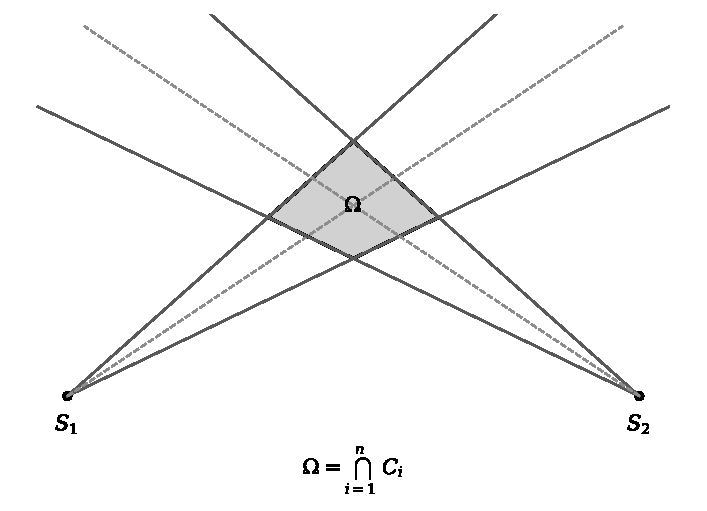
\includegraphics[width=0.58\textwidth]{figures/q1-region-intersection.pdf}
  \caption{多个示向度误差区域的公共交集（角度不按比例）}
  \label{fig:q1-region-intersection}
\end{figure}

\subsubsection{定位区域直径及其求解}

按照题目定义，定位区域的直径为区域内任意两点距离的最大值，即
\begin{equation}
  D=\max_{P,Q\in\Omega}d(P,Q)
   =\max_{P,Q\in\Omega}\|P-Q\|_2.
  \label{eq:q1-diameter-definition}
\end{equation}

由于定位区域闭且有界，距离最大值能够取得。

\noindent\textbf{命题 1：}{\kaishu 凸多边形的直径必由其两个顶点取得，即}
\begin{equation}
  D=\max_{1\leq i,j\leq m}\|V_i-V_j\|_2.
  \label{eq:q1-vertex-diameter}
\end{equation}

\noindent\textbf{证明：}
任取 $P,Q\in\Omega$，写成顶点的凸组合 $P=\sum_i\lambda_iV_i$、$Q=\sum_j\mu_jV_j$，其中系数非负且各自之和为 $1$。由三角不等式，
\begin{equation}
  \|P-Q\|_2
  =\left\|\sum_{i,j}\lambda_i\mu_j(V_i-V_j)\right\|_2
  \leq\max_{i,j}\|V_i-V_j\|_2.
  \label{eq:q1-diameter-proof}
\end{equation}

由于 $\sum_{i,j}\lambda_i\mu_j=1$ 且顶点属于 $\Omega$，任意两点距离不超过最大顶点对距离，
而最远顶点对取得该上界。\hfill$\square$

本文采用旋转卡壳法求解最远顶点对。由旋转卡壳定理~\cite{toussaint1983}，直径端点必属于对踵点对。
对边向量 $E_i=V_{i+1}-V_i$，以
$A(i,j)=|E_i\mathbin{\boldsymbol{\times}}(V_j-V_i)|$ 衡量顶点到该边所在直线的距离；
依次增加 $j$ 至该量不再增大，相等时同时检查两个候选点。两个指标均至多绕多边形一周，
故时间复杂度为 $O(m)$。

\subsubsection{直径圆的覆盖判据}

设旋转卡壳法得到的一组直径端点为 $V_p,V_q$。以线段 $V_pV_q$ 为直径构造圆，下文所称“圆覆盖”均指该圆的闭圆面覆盖。其圆心和半径分别为
\begin{equation}
  O=\frac{V_p+V_q}{2},\qquad r=\frac{D}{2}.
  \label{eq:q1-diameter-circle}
\end{equation}

\noindent\textbf{命题 2：}{\kaishu 直径圆能够覆盖整个定位区域 $\Omega$ 的充分必要条件为}
\begin{equation}
  \max_{1\leq j\leq m}\|V_j-O\|_2\leq\frac{D}{2}.
  \label{eq:q1-circle-criterion}
\end{equation}

\noindent\textbf{证明：}
若圆覆盖区域，必然包含全部顶点；反之，闭圆盘为凸集，包含全部顶点就包含它们的凸包 $\Omega$。\hfill$\square$

直径圆不一定覆盖第三个顶点，如图~\ref{fig:q1-diameter-circle} 所示，因此仍须逐顶点检查
式~\eqref{eq:q1-circle-criterion}；问题二据此改用最小包围圆衡量定位不确定性。

\begin{figure}[H]
  \centering
  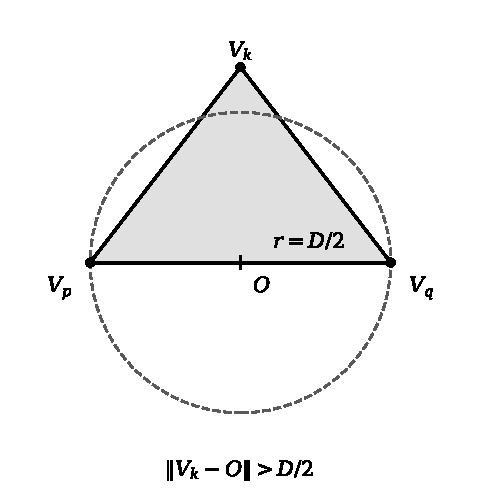
\includegraphics[width=0.52\textwidth]{figures/q1-diameter-circle.pdf}
  \caption{直径圆未覆盖定位区域的反例（长度不按比例）}
  \label{fig:q1-diameter-circle}
\end{figure}

求解过程依次为：求交会多边形、用旋转卡壳计算直径、逐顶点检验直径圆覆盖性。

\subsubsection{建模边界及对后续问题的影响}

问题一按题意求纯角度交会区域 $\Omega$。进一步利用目标圆形区域和成功接收时距离不超过 $1500\ \mathrm m$ 的条件，可得更小的物理可行域

\begin{equation}
  K=\Omega\cap\overline B(O_0,1800)
  \cap\bigcap_{i=1}^{n}\overline B(S_i,1500).
  \label{eq:q1-physical-region}
\end{equation}

其中 $1500\ \mathrm m$ 是有效接收半径的统一上界，$1000\ \mathrm m$ 不构成源与测点间的距离下界。
$K$ 仍为凸集，但圆盘可能截断 $\Omega$ 并形成图~\ref{fig:q1-curved-regions} 所示的圆弧边界。

\begin{figure}[H]
  \centering
  \begin{subfigure}[t]{0.48\textwidth}
    \centering
    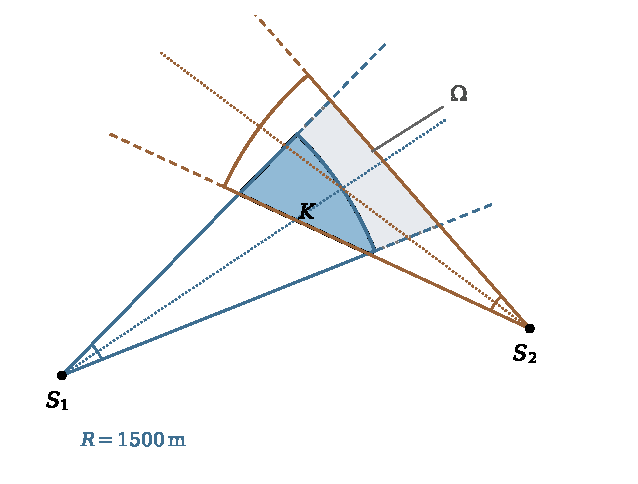
\includegraphics[width=\linewidth]{figures/q1-receive-radius-arc.pdf}
    \caption{两个有限探测扇形交会形成圆弧边界}
  \end{subfigure}\hfill
  \begin{subfigure}[t]{0.48\textwidth}
    \centering
    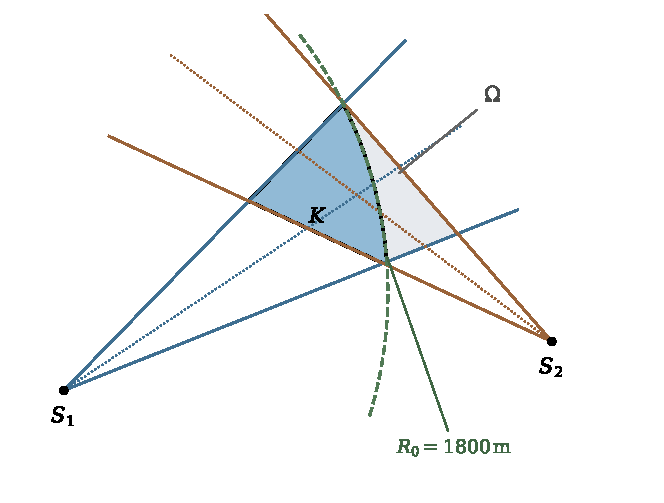
\includegraphics[width=\linewidth]{figures/q1-arena-radius-arc.pdf}
    \caption{目标圆形区域截断交会多边形}
  \end{subfigure}
  \caption{定位区域出现圆弧边界的两种情形（图中长度不按比例）}
  \label{fig:q1-curved-regions}
\end{figure}

圆弧上的直径端点可能不在直线边界交点中。由 $K\subseteq\Omega$，问题一的多边形直径仍是物理
可行域直径的上界。问题二用固定边数的外切正多边形替代圆盘，得到
$K\subseteq\widehat K$ 及
$\operatorname{diam}(K)\leq\operatorname{diam}(\widehat K)$；该外近似保留真实位置并提供保守覆盖判定。

\subsection{问题二的模型建立与求解}

\subsubsection{单次检测后的源位置可行域}

记第一检测点为 $S_1$，其对某全向干扰源测得的示向度为 $\theta_1$，相应误差角区为 $C_1$。题设给出目标圆形区域半径为 $1800\ \mathrm{m}$，全向干扰源的实际有效接收半径 $R_s$ 满足
\begin{equation}
  R_s\in[R_{\min},R_{\max}]=[1000,1500]\ \mathrm{m}.
\end{equation}

因为 $S_1$ 已获得示向度，真实源位置 $X$ 必满足 $\|X-S_1\|_2\leq R_s\leq R_{\max}$。因此，式~\eqref{eq:q1-physical-region} 在单次观测下具体化为
\begin{equation}
  K_1=C_1\cap\overline B(O_0,1800)
  \cap\overline B(S_1,R_{\max}).
  \label{eq:q2-physical-region}
\end{equation}

为处理式~\eqref{eq:q2-physical-region} 中的圆弧边界，构造包含原圆盘的固定粗外包。对以 $A$ 为圆心、$R$ 为半径的圆盘，取 $N$ 个等分单位法向量
\begin{equation}
  n_k=\left(\cos\frac{2k\pi}{N},
  \sin\frac{2k\pi}{N}\right)^{\mathsf T},
  \qquad k=0,1,\ldots,N-1,
\end{equation}

并以相应切线半平面之交构造外切正多边形
\begin{equation}
  \widehat B_{\mathrm{out}}^{(N)}(A,R)
  =\bigcap_{k=0}^{N-1}
  \left\{Y:n_k^{\mathsf T}(Y-A)\leq R\right\}.
  \label{eq:q2-outer-polygon}
\end{equation}

本文采用当前程序的固定粗外包构造。取 $N=24$，将目标圆盘和接收上界圆盘分别替换为式~\eqref{eq:q2-outer-polygon} 的外切正多边形，再加入角区 $C_1$ 的两个半平面约束。将这些半平面记为 $\mathcal H_N$，其交集即为后续计算使用的源位置区域：
\begin{equation}
  \widehat K_1=C_1
  \cap\widehat B_{\mathrm{out}}^{(N)}(O_0,1800)
  \cap\widehat B_{\mathrm{out}}^{(N)}(S_1,R_{\max})
  =\bigcap_{H\in\mathcal H_N}H.
  \label{eq:q2-source-region}
\end{equation}

圆盘与固定外切正多边形的几何关系如图~\ref{fig:q2-k1-outer-approx} 所示。正多边形的每条边均与圆相切，因此圆盘完全包含在多边形内；多边形顶点方向处的径向外扩最大。

\begin{figure}[H]
  \centering
  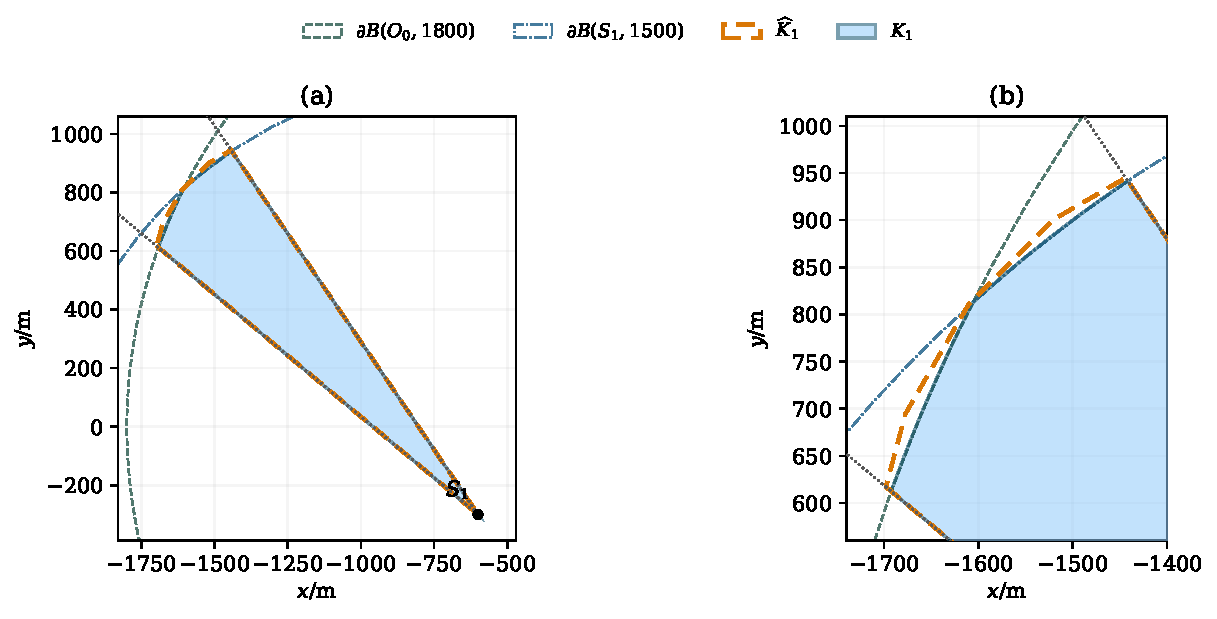
\includegraphics[width=0.64\textwidth]{figures/q2-k1-outer-approx.pdf}
  \caption{外切正多边形局部示意：$T_-,T_+$ 为切点，$V$ 为切线交点，$\Delta_{\mathrm{out}}$ 为最大径向外扩（角度放大，计算取 $N=24$）}
  \label{fig:q2-k1-outer-approx}
\end{figure}

每个切线半平面都包含原圆盘，且角区约束不变，故 $K_1\subseteq\widehat K_1$。这一外近似避免误删真实源，并将圆弧约束转为可求交、枚举顶点及检查覆盖的线性半平面约束。

当 $N=24$ 时，固定粗外包的最大径向外扩量为
\begin{equation}
  \Delta_{\mathrm{out}}(R,N)
  =R\left(\sec\frac{\pi}{N}-1\right).
\end{equation}

半径为 $1800\ \mathrm{m}$ 和 $1500\ \mathrm{m}$ 的圆形区域对应值分别约为 $15.532\ \mathrm{m}$ 和 $12.943\ \mathrm{m}$。这是固定 $24$ 边粗外包的最大径向误差，全部计算均保持这一外包形式。程序中将理论示向度误差 $1^\circ$ 扩大为 $1.005^\circ$，用于降低边界浮点误差导致真实源被错误排除的风险。本文后续模型均沿用这一固定粗外包口径。

\subsubsection{定位不确定性半径}

问题一已证明，以区域直径端点作直径圆时，该圆不一定覆盖整个定位区域。故问题二统一采用最小包围圆尺度描述定位不确定性。对任意非空有界集合 $A$，定义其定位不确定性半径为
\begin{equation}
  \rho(A)=\min_{Q\in\mathbb R^2}
  \max_{Y\in A}\|Y-Q\|_2.
  \label{eq:q2-mec-radius}
\end{equation}

由区域内任意直径端点都必须同时被包围圆覆盖，有
\begin{equation}
  \rho(A)\geq\frac{\operatorname{diam}(A)}{2}.
  \label{eq:q2-diameter-mec}
\end{equation}

直径圆能够覆盖区域时取等号，否则最小包围圆半径更大。记第一次观测后的不确定性半径为 $R_0=\rho(\widehat K_1)$。

设 $\widehat K_1=\operatorname{conv}\{V_1,\ldots,V_m\}$。由问题一的圆覆盖判据，只需对顶点求最小包围圆。遍历单点退化圆、两点直径圆与三个不共线点的外接圆，保留满足
\begin{equation}
  \max_{1\leq l\leq m}\|V_l-Q\|_2\leq r+\tau
  \label{eq:q2-mec-cover-test}
\end{equation}

的候选圆 $(Q,r)$，再取半径最小者；$\tau$ 为数值容差。三点组合有 $O(m^3)$ 个，每圆检查 $m$ 个顶点，故最坏时间复杂度为 $O(m^4)$，适用于本题较少的顶点数。

\subsubsection{第二检测点的候选区域}

若要求无论真实源位于当前可行域中何处、其有效接收半径在题设区间中取何值，第二测点 $s$ 都能收到信号，则必须有
\begin{equation}
  \mathcal F_g(\widehat K_1)
  =\left\{s:\max_{X\in\widehat K_1}
  \|s-X\|_2\leq R_{\min}\right\}.
  \label{eq:q2-guaranteed-region}
\end{equation}

由问题一的圆覆盖判据，一个以 $s$ 为圆心、半径为 $R_{\min}$ 的圆覆盖全部顶点，就覆盖整个 $\widehat K_1$，因此
\begin{equation}
  \mathcal F_g(\widehat K_1)
  =\bigcap_{j=1}^{m}\overline B(V_j,R_{\min}).
  \label{eq:q2-guaranteed-vertices}
\end{equation}

以各 $V_j$ 为圆心构造半径 $R_{\min}$ 的内接正 $72$ 边形，逐一求交得到保证接收域 $\widehat{\mathcal F}_g$。为使输出测点确实可行，此处采用与源区域相反的内近似方向，满足

\begin{equation}
  \widehat{\mathcal F}_g
  \subseteq\mathcal F_g(\widehat K_1)
  \subseteq\mathcal F_g(K_1).
  \label{eq:q2-guaranteed-inclusion}
\end{equation}

其最大径向收缩量为
\begin{equation}
  R_{\min}\left(1-\cos\frac{\pi}{72}\right)
  \approx0.952\ \mathrm{m}.
\end{equation}

故落在 $\widehat{\mathcal F}_g$ 中的测点对当前全向距离接收模型具有保守的接收保证。若 $\widehat{\mathcal F}_g$ 为空，只说明当前内近似未能给出可认证的保证接收点，不由此断言理论保证域必然为空。

另一方面，若只要求存在某个相容源位置使测点可能收到信号，则计算可能接收域
\begin{equation}
  \mathcal F_p
  =\left\{s:\operatorname{dist}(s,\widehat K_1)
  \leq R_{\max}\right\}
  =\widehat K_1\oplus\overline B(O_0,R_{\max}),
  \label{eq:q2-possible-region}
\end{equation}

其中 $\oplus$ 表示 Minkowski 和，即将源区域向外扩张 $R_{\max}$。沿 $72$ 个支撑方向建立半平面可得其外近似 $\widehat{\mathcal F}_p$，用于辅助展示可能接收范围。题目所求第二检测点的候选区域取保证接收域 $\widehat{\mathcal F}_g$，三类区域的关系见图~\ref{fig:q2-reception-regions}。

\begin{figure}[H]
  \centering
  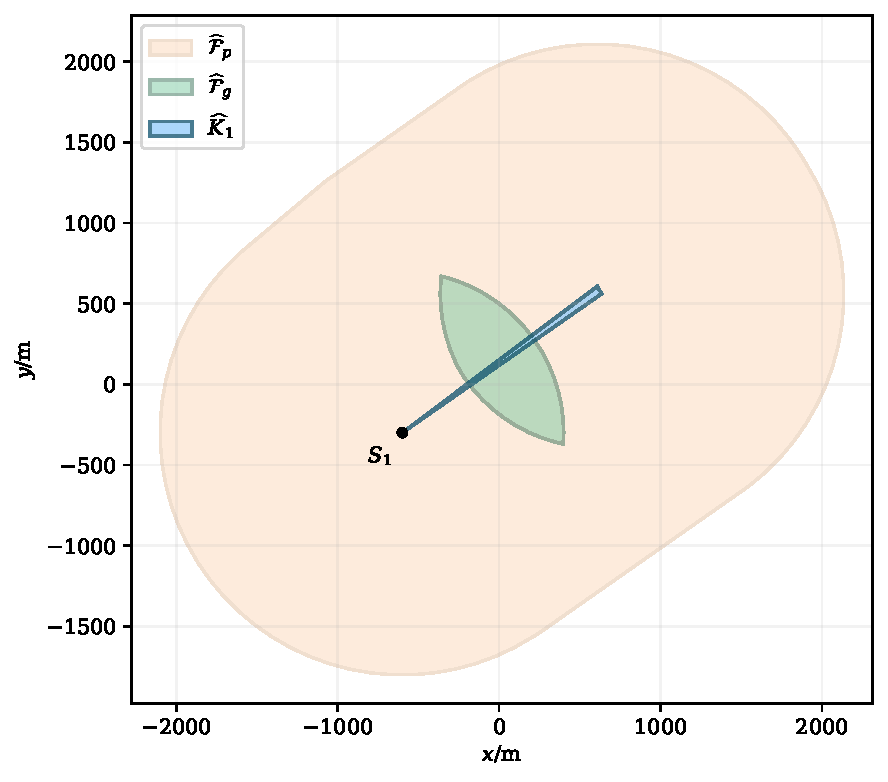
\includegraphics[width=0.68\textwidth]{figures/q2-reception-regions.pdf}
  \caption{源位置区域 $\widehat K_1$、保证接收域 $\widehat{\mathcal F}_g$ 与可能接收域 $\widehat{\mathcal F}_p$ 的关系}
  \label{fig:q2-reception-regions}
\end{figure}

\subsubsection{二次定位不确定性半径的场景预测与行动时间}

选点时尚未获得第二次检测结果，因此通过有限源位置和示向误差场景，预测候选点对定位区域的收缩效果。

记 $\widehat K_1$ 为仅利用第一次检测和物理边界得到的源位置区域，首先离散化干扰源的可能位置。设 $\widehat K_1$ 的顶点按边界顺序为 $V_1,\ldots,V_m$，并令 $V_{m+1}=V_1$。构造三类原始场景：$m$ 个顶点 $V_i$、$m$ 个边中点 $M_i=(V_i+V_{i+1})/2$，以及一个顶点均值中心 $G=m^{-1}\sum_iV_i$，共 $2m+1$ 个点。若其总数不超过 $8$，则全部保留；否则按照固定顺序
\begin{equation}
  V_1,M_1,V_2,M_2,\ldots,V_m,M_m,G
\end{equation}

在序列中等间隔选取 $8$ 个索引，得到有限源位置场景集 $\mathcal S_A$。图~\ref{fig:q2-source-scenarios} 以五边形为例展示了三类原始点及最终保留的 $8$ 个选点。

\begin{figure}[H]
  \centering
  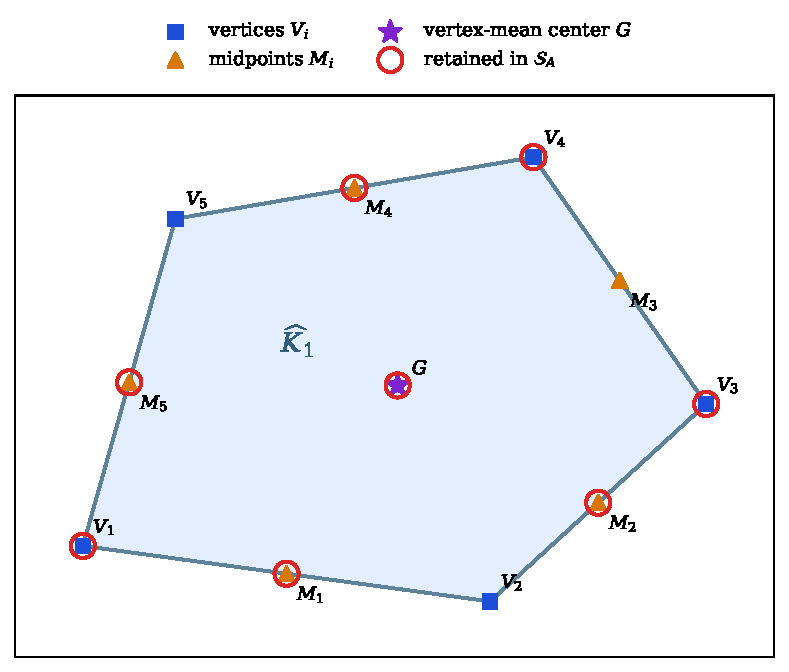
\includegraphics[width=0.66\textwidth]{figures/q2-source-scenarios.pdf}
  \caption{有限源位置场景的构造示例（红色空心圆表示由三类原始点确定性下采样后保留的场景）}
  \label{fig:q2-source-scenarios}
\end{figure}

其次讨论二次检测误差。对假定源位置 $X\in\mathcal S_A$ 和候选检测点 $s$，将在该场景中从 $s$ 指向 $X$ 的无误差方位角记为 $\theta(s,X)$，取有限误差场景集
\begin{equation}
  \mathcal E=\{-\varepsilon,0,+\varepsilon\},
  \qquad \varepsilon=1.005^\circ
\end{equation}

对于 $e\in\mathcal E$，相应的假想二次示向度为
\begin{equation}
  \widehat\theta_2(s;X,e)=\theta(s,X)+e.
\end{equation}

当 $5<\|s-X\|_2\leq R_{\max}$ 且假想示向度有效时，可以得到新的误差角区。因此，该场景对应的预测更新区域为
\begin{equation}
  \widehat K_2(s;X,e)
  =\widehat K_1
  \cap\widehat B_{\mathrm{out}}^{(N)}(s,R_{\max})
  \cap C\bigl(s,\widehat\theta_2(s;X,e),\varepsilon\bigr),
  \label{eq:q2-posterior-region}
\end{equation}

其中 $C(s,\theta,\varepsilon)$ 表示以 $s$ 为顶点、方向为 $\theta$、左右误差界为 $\varepsilon$ 的角区；新增接收圆形区域仍采用第~5.2.1 节相同的固定 $N=24$ 边外切正多边形，全部约束均保持固定粗外包形式。此时 $\rho(\widehat K_2)$ 即为该场景下预测的二次定位不确定性半径。

当 $\|s-X\|_2\leq5\ \mathrm{m}$ 时，题设规定测向机可能返回近距离结果而不给出示向度，此时以 $\min\{5,R_0\}$ 作为定位不确定性半径的保守上界，其中 $R_0=\rho(\widehat K_1)$。综合近距离与有效示向度两类假想结果，定义二次定位不确定性半径的单场景预测值为
\begin{equation}
  r_2(s;X,e)=
  \begin{cases}
    \min\{5,R_0\}, & \|s-X\|_2\leq5,\\
    \rho\bigl(\widehat K_2(s;X,e)\bigr),
      & 5<\|s-X\|_2\leq R_{\max}.
  \end{cases}
\end{equation}

若 $s\notin\mathcal F_g(\widehat K_1)$，则由于真实源位置及其实际接收半径未知，第二次检测还可能返回无信号。当前模型不利用无信号结果进一步排除位置，而保守地认为定位区域未发生收缩，将该分支的定位不确定性半径预测值记为 $R_0$。计算时通过 $\widehat K_1$ 的顶点最大距离检验式~\eqref{eq:q2-guaranteed-region} 的保证接收条件。由此定义二次定位不确定性半径的有限场景最坏预测值
\begin{equation}
  R_{\mathrm{wc}}(s)
  =\max\left(
  \left\{
  r_2(s;X,e):
  X\in\mathcal S_A,\ e\in\mathcal E,\
  \|s-X\|_2\leq R_{\max}
  \right\}
  \cup\mathcal R_{\mathrm{no}}(s)
  \right),
  \label{eq:q2-worst-radius}
\end{equation}

其中
\begin{equation}
  \mathcal R_{\mathrm{no}}(s)=
  \begin{cases}
    \varnothing, & s\in\mathcal F_g(\widehat K_1),\\
    \{R_0\}, & s\notin\mathcal F_g(\widehat K_1).
  \end{cases}
\end{equation}

$R_{\mathrm{wc}}(s)$ 越小，表示所检查不利场景下的定位不确定性越小；它是有限场景预测值，不构成连续源位置和误差范围上的最坏情况保证。

问题二中机器狗由 $S_1$ 直接前往 $s$，且检测频道不变，故行动时间为
\begin{equation}
  T(s)=\frac{\|s-S_1\|_2}{v}+\tau_{\mathrm{meas}}
  =\frac{\|s-S_1\|_2}{5}+5.
  \label{eq:q2-action-time}
\end{equation}

若该模型在后续问题中从其他位置或其他频道调用，则再将当前位置替换为 $p_c$，并在频道不同时加入 $1\ \mathrm{s}$ 换频时间。

下面分别采用有限离散评分和连续 Fisher 信息搜索，在候选区域内选择具体检测点。

\subsubsection{方案一：候选区域内的有限离散候选点综合评分策略}

方案一生成并筛选有限离散候选点。其基本思路是先依据首次检测方向和源位置区域的几何结构布置有限候选点，再逐点评价行动时间与二次定位不确定性，从中选出综合评分最小的第二检测点。

将首次检测所得示向度由度转换为弧度 $\vartheta_1=\pi\theta_1/180$，记其方向及左法向分别为
\begin{equation}
  u_1=(\cos\vartheta_1,\sin\vartheta_1)^{\mathsf T},
  \qquad
  n_1=(-\sin\vartheta_1,\cos\vartheta_1)^{\mathsf T}.
\end{equation}

首先构造前向---横向组合候选点
\begin{equation}
  s=S_1+d u_1+\ell n_1,
  \label{eq:q2-directional-candidates}
\end{equation}

其中
\begin{equation}
  d\in\{100,250,500,750\}\ \mathrm{m},
  \qquad
  \ell\in\{0,\pm d/2,\pm d\}.
\end{equation}

前向移动用于接近可能的干扰源，横向移动用于打破两次检测所得示向度近似共线的不利几何。此外，在 $\widehat K_1$ 的最小包围圆中心 $Q_0$ 附近按 $250,500,750\ \mathrm{m}$ 三个半径和八个方向生成环状候选，并加入 $S_1$ 与 $Q_0$ 的中点以及保证接收内近似的顶点均值中心两个特殊点，得到确定性有限候选集 $\mathcal C_A$。这些点不预先用可能接收域裁剪，其中满足保证接收条件的候选子集为
\begin{equation}
  \mathcal C_A^g
  =\left\{s\in\mathcal C_A:
  \max_{X\in\widehat K_1}\|s-X\|_2\leq R_{\min}\right\}
  =\mathcal C_A\cap\mathcal F_g(\widehat K_1).
  \label{eq:q2-discrete-guaranteed-candidates}
\end{equation}

图~\ref{fig:q2-discrete-candidates} 给出了有限离散候选点的构造示例。左图展示候选点在可能接收域、保证接收域和源位置区域中的整体分布；右图放大显示前向---横向点、中心环状点和两个特殊点，红色空心圆标出落入保证接收内近似 $\widehat{\mathcal F}_g$ 的候选点。

\begin{figure}[H]
  \centering
  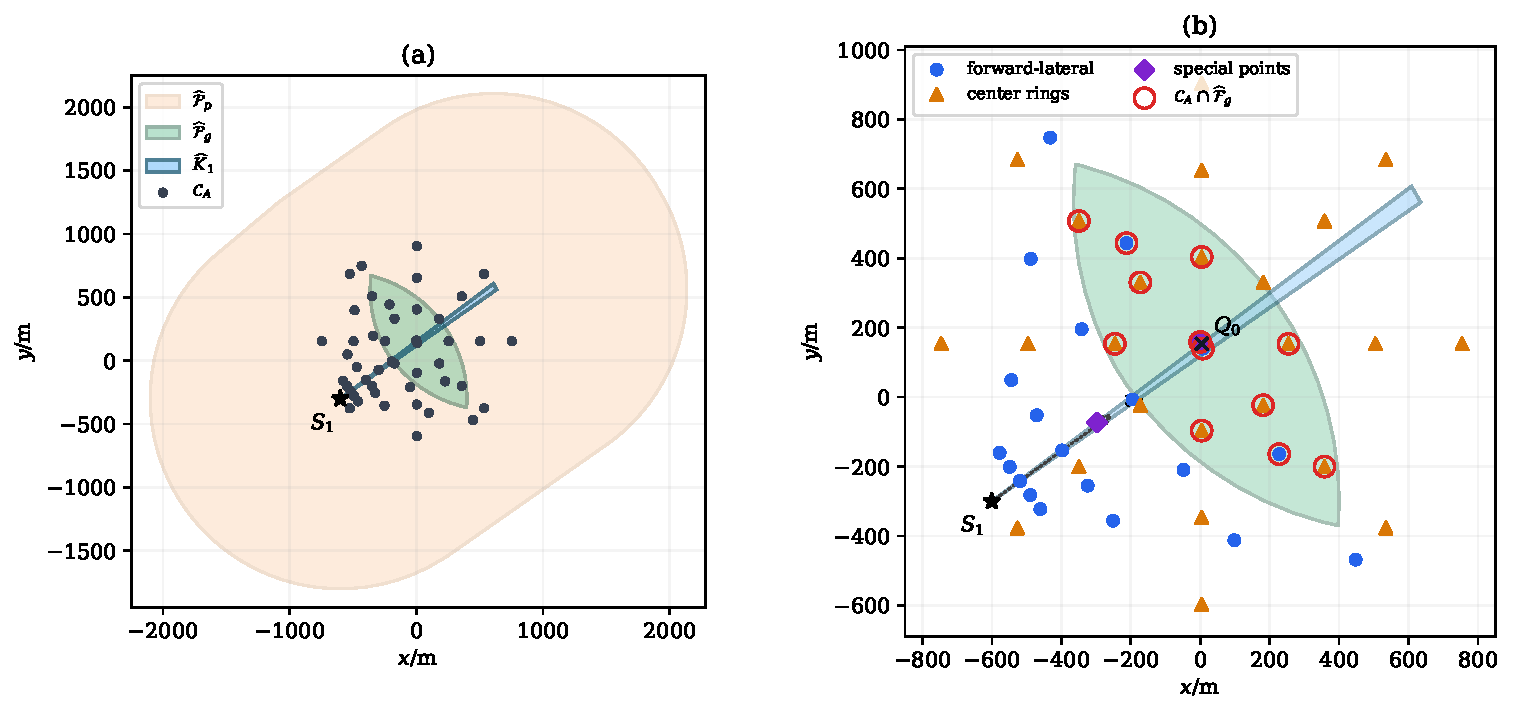
\includegraphics[width=0.94\textwidth]{figures/q2-discrete-candidates.pdf}
  \caption{候选区域内有限离散候选点的构造与筛选示意图}
  \label{fig:q2-discrete-candidates}
\end{figure}

对有限离散候选集 $\mathcal C_A$ 中的每个候选点，为同时衡量行动时间和定位不确定性，定义综合评分
\begin{equation}
  J(s)=T(s)+\lambda_RR_{\mathrm{wc}}(s),
  \qquad \lambda_R=0.5\ \mathrm{s/m}.
  \label{eq:q2-discrete-score}
\end{equation}

$\lambda_R$ 是平衡行动时间与定位不确定性半径的权重超参数，单位为 $\mathrm{s/m}$；本文取 $0.5\ \mathrm{s/m}$，其数值可按两项目标的相对偏好调整，并非题设常数。若 $\mathcal C_A^g$ 非空，则方案一选出的候选点为
\begin{equation}
  s_A=\operatorname*{arg\,min}_{s\in
  \mathcal C_A^g}J(s).
  \label{eq:q2-baseline-choice}
\end{equation}

若 $\mathcal C_A^g$ 为空，则退回全部 $\mathcal C_A$ 中求 $J(s)$ 最小的点，并通过式~\eqref{eq:q2-worst-radius} 中的无信号分支惩罚接收风险。该方案的最优性仅针对当前有限离散候选集、有限源场景和式~\eqref{eq:q2-discrete-score} 的综合评分成立。

\subsubsection{方案二：保证候选区域内的连续 Fisher 信息选点策略}

方案二是在保证接收候选区域 $\widehat{\mathcal F}_g$ 内连续改变测点坐标并产生候选点的策略。有限离散候选可能遗漏相邻点之间交会几何更好的位置，因此以 Fisher 信息矩阵衡量局部方位观测对源位置的辨识能力~\cite{fisher1922}。对检测点 $S_i=(x_i,y_i)$ 和源位置 $X=(x,y)$，理想方位观测为
\begin{equation}
  h_i(X)=\operatorname{atan2}(y-y_i,x-x_i),
\end{equation}

其中 $\operatorname{atan2}$ 为四象限反正切函数，示向度统一转换至 $[0,2\pi)$。

其对 $X$ 的梯度为
\begin{equation}
  q_i(X)=\nabla_X h_i(X)
  =\frac{1}{d_i^2}
  \begin{bmatrix}
    -(y-y_i)\\ x-x_i
  \end{bmatrix},
  \qquad d_i=\|X-S_i\|_2.
\end{equation}

为构造信息量替代目标，暂将两次角度扰动视为相互独立且具有相同局部方差 $\sigma_\theta^2$，则
\begin{equation}
  \mathcal I(s;X)
  =\frac{1}{\sigma_\theta^2}
  \left(q_1q_1^{\mathsf T}+q_2q_2^{\mathsf T}\right),
  \qquad S_2=s.
  \label{eq:q2-fim}
\end{equation}

设从两个检测点指向源的视线夹角为 $\phi(s;X)$。利用二维恒等式 $\det(aa^{\mathsf T}+bb^{\mathsf T})=(a_1b_2-a_2b_1)^2$，由式~\eqref{eq:q2-fim} 直接得
\begin{equation}
  \det\mathcal I(s;X)
  =\frac{\sin^2\phi(s;X)}
  {\sigma_\theta^4d_1^2d_2^2}.
  \label{eq:q2-fim-determinant}
\end{equation}

式~\eqref{eq:q2-fim-determinant} 表明，两条视线近似平行时，两次示向度提供的方向约束近似重复，交会定位结果对角度误差较为敏感；在距离相当时，较大的交会角通常提供更多定位信息；而观测距离过大会放大角度误差所导致的定位不确定性。

略去对所有候选点相同的 $\sigma_\theta^{-4}$，引入仅用于调整数值尺度的常数 $\kappa=10^{12}$，并用行动时间归一化，定义
\begin{equation}
  \Phi(s;X)=
  \frac{\kappa\sin^2\phi(s;X)}
  {d_1^2d_2^2T(s)}.
\end{equation}

当 $d_2\leq5\ \mathrm{m}$ 时，检测将进入近距离分支，不再适用常规示向度 Fisher 指标，因而在数值搜索中使用有界的有利近似 $\Phi(s;X)=\kappa/(25d_1^2T(s))$。又因首次检测已获得有效示向度，Fisher 场景构造时排除 $d_1\leq5\ \mathrm{m}$ 的退化点。
对 $\widehat K_1$ 每条边上的若干等分点及区域中心构造确定性场景集 $\mathcal S_F$，再取
\begin{equation}
  \Phi_{\mathrm{rob}}(s)
  =\min_{X\in\mathcal S_F}\Phi(s;X),
  \label{eq:q2-robust-fim}
\end{equation}

表示当前所检查源位置中的最小单位时间信息量。

记方案一选点的行动时间为 $T_A=T(s_A)$。为同时考察“较快到达”与“允许走得更远以改善交会几何”的情形，额外给出三档行动时间余量 $b\in\{15,30,60\}\ \mathrm{s}$，分别求解
\begin{equation}
  s_F^{(b)}
  =\operatorname*{arg\,max}_{s\in\widehat{\mathcal F}_g}
  \Phi_{\mathrm{rob}}(s),
  \qquad T(s)\leq T_A+b.
  \label{eq:q2-fim-budget}
\end{equation}

每档最多产生一个候选点，共同反映额外行动时间与交会几何之间的权衡。

求解时从保证域中心、边界顶点、边中点及离散候选中选取多个初始点，在 $16$ 个方向上进行投影模式搜索。试探点越出 $\widehat{\mathcal F}_g$ 时将其投影回可行多边形；若没有找到更优点，则将步长减半，直至步长由 $200\ \mathrm{m}$ 缩小至 $2\ \mathrm{m}$，或达到迭代次数、求解时间等预设上限；达到上限时返回已经搜索到的最优可行点。
\subsubsection{统一评价与最终选点}

方案一的 $J(s)$ 与方案二的 $\Phi_{\mathrm{rob}}(s)$ 量纲和物理含义均不同，不能直接根据两个数值判断测点优劣。因此，Fisher 信息优化只用于在保证接收区域内搜索可能具有较好交会几何的连续测点坐标，并不直接决定最终测点。三档预算所得候选均重新使用式~\eqref{eq:q2-worst-radius} 和式~\eqref{eq:q2-action-time} 计算
\begin{equation}
  \bigl(R_{\mathrm{wc}}(s),T(s),J(s)\bigr).
\end{equation}

在实际执行时，首先保留满足 $T(s)\leq T_A+30\ \mathrm{s}$ 的连续候选。$60\ \mathrm{s}$ 档产生的候选仅在其实际行动时间不超过 $T_A+30\ \mathrm{s}$ 时纳入最终可执行集。对每个保留的连续候选点，定义有序评价向量
\begin{equation}
  \boldsymbol z(s)=\left(R_{\mathrm{wc}}(s),T(s),
  -\Phi_{\mathrm{rob}}(s),s_x,s_y\right).
\end{equation}

按 $\boldsymbol z(s)$ 从左到右逐级比较：优先选择 $R_{\mathrm{wc}}$ 小的点，相同时比较行动时间，再比较信息量和坐标，得到连续代表点 $s_F$。

另在离散选点与三档连续候选组成的集合 $\mathcal C$ 中，保留时间与定位半径均不被其他点同时改善的非支配候选，供两目标权衡分析；最终执行仍按下述规则决定。

最终执行点只在方案一选点 $s_A$ 和连续代表点 $s_F$ 之间，按照“定位不确定性半径的最坏预测值优先、行动时间次之”的规则选取
\begin{equation}
  s^*=\operatorname*{lex\,arg\,min}_{s\in\{s_A,s_F\}}
  \left(R_{\mathrm{wc}}(s),T(s),s_x,s_y\right).
  \label{eq:q2-final-choice}
\end{equation}

其中 $\mathrm{lex}$ 表示上述逐级比较顺序，坐标仅用于消除并列结果。若连续优化不可用，则令 $s^*=s_A$。

\subsubsection{候选区域、选点策略总结及推广}

综上，实际候选区域为保证接收内近似 $\widehat{\mathcal F}_g$，推荐点由离散与连续方案统一复评分后按式~\eqref{eq:q2-final-choice} 选出。离散保证候选为空时回退至全部离散候选，并计入无信号风险；连续方案仅在保证域非空时运行。

这一策略可由“已有一个检测点”直接推广至“已有多个检测点”：用全部有效示向度约束更新当前区域 $\widehat K_n$，再以 $\widehat K_n$ 重新构造候选区域并选择第 $n+1$ 个检测点。问题三直接利用该递推方法实现全向干扰源的连续定位；问题四保留多观测区域更新和定位不确定性评价，但由于定向干扰源在距离足够近时仍可能因辐射方向不符而无信号，需将下一检测点扩展为从多个方向接近的探测点。

\subsection{问题三的模型建立与求解}

问题三将前两问扩展为由模拟器反馈驱动的连续决策过程，包括八点扫描、观测更新、批量补充定位、
清除路线排序和逐源清除。

\subsubsection{执行状态与行动时间}

记当前位置、检测频道和累计虚拟时间为 $p,h,t$；频道集合分为已发现未清除、无源和已清除三类
$\mathcal C_f,\mathcal C_a,\mathcal C_c$。每个已发现频道保存区域 $\widehat K_j$、最小包围圆
$(c_j,r_j)$ 和清除队列 $Q_j$ 等状态。

机器狗每次只发出进入、检测、清除或退出中的一个动作，收到并处理该动作的响应后才生成下一动作。设机器狗从 $p$ 移动到 $s$，速度为 $v=5\ \mathrm{m/s}$，换频时间为 $\tau_{\mathrm{sw}}=1\ \mathrm{s}$，检测时间为 $\tau_{\mathrm{meas}}=5\ \mathrm{s}$，则检测动作的虚拟时间为
\begin{equation}
  T_{\mathrm{measure}}(p,h;s,j)
  =\frac{\|s-p\|_2}{v}
  +\tau_{\mathrm{sw}}\mathbf 1_{\{h\ne j\}}
  +\tau_{\mathrm{meas}}.
  \label{eq:q3-measure-time}
\end{equation}

若在 $s$ 对频道 $j$ 执行清除，光电操作耗时 $3\ \mathrm{s}$，清除成功时激光发射再耗时 $2\ \mathrm{s}$。记清除结果为 $b\in\{0,1\}$，其中 $b=1$ 表示成功，则
\begin{equation}
  T_{\mathrm{clear}}(p;s,b)
  =\frac{\|s-p\|_2}{v}+3+2b.
  \label{eq:q3-clear-time}
\end{equation}

两式用于后续选点与排序，现实计算时间不计入虚拟行动时间。

\subsubsection{八个等角驻留点的初始扫描}

记目标分布区域为 $\mathcal D=\overline B(O_0,1800)$。

由于每个全向干扰源的有效接收半径至少为 $1000\ \mathrm{m}$，只要扫描驻留点集合对 $\mathcal D$ 的覆盖半径不超过 $1000\ \mathrm{m}$，就能保证每个源至少在一个驻留点被发现。本文取环半径 $a=960\ \mathrm{m}$，在圆周上设置八个等角驻留点
\begin{equation}
  P_k=O_0+a
  \left(\cos\frac{k\pi}{4},\sin\frac{k\pi}{4}\right),
  \qquad k=0,1,\ldots,7.
  \label{eq:q3-eight-points}
\end{equation}

机器狗从原点依次访问 $P_0,\ldots,P_7$，在每点先检测当前频道，再检测其他频道。
布局、顺序及保证接收圆如图~\ref{fig:q3-eight-point-scan} 所示。

\begin{figure}[H]
  \centering
  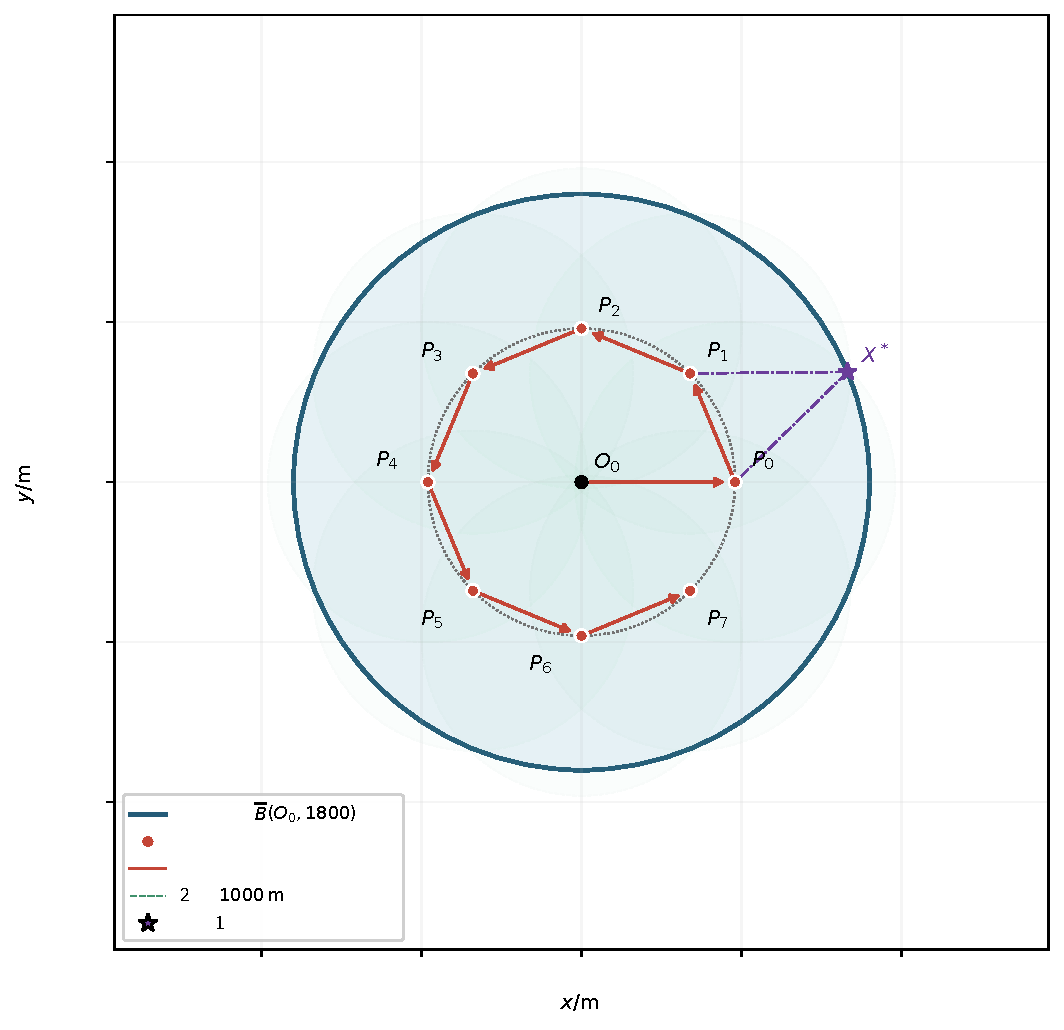
\includegraphics[width=0.78\textwidth]{figures/q3-eight-point-scan.pdf}
  \caption{八点扫描及保证接收覆盖：箭头表示访问顺序，$X^*$ 为最不利边界位置}
  \label{fig:q3-eight-point-scan}
\end{figure}

\noindent\textbf{命题 3：}{\kaishu 式~\eqref{eq:q3-eight-points} 给出的八个驻留点能够以小于 $1000\ \mathrm{m}$ 的覆盖半径覆盖整个目标圆形区域 $\mathcal D$。}

\noindent\textbf{证明：}
任取 $X\in\mathcal D$，以 $O_0$ 为极点写成极坐标 $(\rho,\theta)$，其中 $0\leq\rho\leq1800$。八个驻留点将圆周方向等分，因此必存在某个 $P_k$，使 $X$ 与 $P_k$ 的极角差 $\Delta$ 满足 $|\Delta|\leq\pi/8$。由余弦定理，
\begin{equation}
  \|X-P_k\|_2^2
  =\rho^2+a^2-2a\rho\cos\Delta.
  \label{eq:q3-cover-distance}
\end{equation}

该式对 $\rho$ 为凸函数，并随 $|\Delta|$ 增大，故只需比较圆心与目标圆周角平分方向。代入 $a=960$ 得
\begin{equation}
  \begin{aligned}
    d_{\mathrm{cov}}
    &=\max_{X\in\mathcal D}\min_{0\leq k\leq7}\|X-P_k\|_2,\\
    &=\max\left\{960,
      \sqrt{1800^2+960^2-2(1800)(960)\cos(\pi/8)}
      \right\},\\
    &\approx984.212\ \mathrm{m}<1000\ \mathrm{m}.
  \end{aligned}
\end{equation}

故八点布局覆盖整个目标区域。\hfill$\square$

近距离结果立即原地清除；有效示向度用于更新区域；无信号时继续扫描。

设频道 $j$ 已在位置 $S_{j,1},\ldots,S_{j,m}$ 获得示向度 $\theta_{j,1},\ldots,\theta_{j,m}$。沿用问题一的角度误差半平面交，并加入问题二的目标圆形区域与接收距离上界，实时计算使用的源位置外近似为
\begin{equation}
  \widehat K_j^{(m)}
  =\widehat B_{\mathrm{out}}^{(N_3)}(O_0,1800)
  \cap\bigcap_{i=1}^{m}
  \left[
  C(S_{j,i},\theta_{j,i},\varepsilon)
  \cap\widehat B_{\mathrm{out}}^{(N_3)}(S_{j,i},1500)
  \right],
  \qquad N_3=16.
  \label{eq:q3-region-update}
\end{equation}

其中 $\varepsilon=1.005^\circ$，实时圆盘外切多边形边数 $N_3=16$。
$\widehat K_j^{(m)}$ 是包含真实源的有界凸多边形，且新增观测只会加入约束，因此
\begin{equation}
  \widehat K_j^{(m+1)}\subseteq\widehat K_j^{(m)}.
  \label{eq:q3-nested-regions}
\end{equation}

随后计算 $\widehat K_j^{(m)}$ 的最小包围圆
\begin{equation}
  \widehat K_j^{(m)}\subseteq\overline B(c_j,r_j),
  \qquad r_j=\rho\bigl(\widehat K_j^{(m)}\bigr).
  \label{eq:q3-mec}
\end{equation}

对扫描中已经发现的频道，记候选扫描点 $P_k$ 相对当前区域中心与已有第 $i$ 个检测点形成的夹角为
\begin{equation}
  \alpha_{j,i}(P_k)
  =\angle\bigl(c_j-S_{j,i},c_j-P_k\bigr),
  \qquad
  \alpha_j(P_k)=\max_i\alpha_{j,i}(P_k).
\end{equation}

若 $r_j\leq15\ \mathrm{m}$ 或 $\alpha_j(P_k)<30^\circ$，则跳过重复检测；否则顺路补充示向度。
该规则只减少低价值检测，不作为最优性结论。

由扫描覆盖结论，八点扫描后仍未发现的频道可归入 $\mathcal C_a$；已发现未清除及已清除频道分别归入 $\mathcal C_f,\mathcal C_c$。三类互不相交，合起来包含全部 $20$ 个频道。

\subsubsection{批量补充定位与停止规则}

扫描阶段结束后，暂不立即逐个往返清除，而是先把所有已发现源处理成有限清除队列。设当前尚未入队的频道集合为 $\mathcal U$，策略按
\begin{equation}
  j^*=\operatorname*{arg\,min}_{j\in\mathcal U}\|p-c_j\|_2
  \label{eq:q3-nearest-source}
\end{equation}

选取距当前位置最近的源作为暂定的下一处理对象。

按定位半径处理：$r_{j^*}\leq19.9\ \mathrm m$ 时将中心加入可靠清除队列；
$19.9<r_{j^*}\leq40\ \mathrm m$ 时加入中心及保底清除点；$r_{j^*}>40\ \mathrm m$ 且补充次数
小于 $M=2$ 时选择新检测点。

补充检测沿用问题二，并按真实响应更新区域；每源最多两次。达到上限后转入有限保底清除队列。
$40\ \mathrm{m}$ 只表示可先试中心并继续保底点，不是中心可靠清除条件。

\subsubsection{开放式旅行商清除顺序}

所有已发现源均形成清除队列后，取各队列的首点，即最小包围圆中心 $c_1,\ldots,c_n$，建立完全图，边权为欧氏距离
\begin{equation}
  d_{ij}=\|c_i-c_j\|_2.
\end{equation}

清除结束后无需返回起点，因此采用开放式旅行商路径而非闭合回路。程序使用 Held--Karp 动态规划的开放式变体求中心之间的最短访问顺序~\cite{heldkarp1962}。对任意非空中心下标集合 $A\subseteq\{1,\ldots,n\}$ 及 $j\in A$，定义
\begin{equation}
  F(A,j)=\text{恰好访问 $A$ 中全部中心且以 $c_j$ 结束的最短内部路径长度}.
\end{equation}

因为路径起点可取 $A$ 中任一中心，初值和递推式为
\begin{equation}
  F(\{j\},j)=0,
  \qquad
  F(A,j)=\min_{i\in A\setminus\{j\}}
  \left[F(A\setminus\{j\},i)+d_{ij}\right].
  \label{eq:q3-held-karp}
\end{equation}

最终中心内部路径长度为
\begin{equation}
  L_{\mathrm{TSP}}
  =\min_{1\leq j\leq n}F(\{1,\ldots,n\},j),
  \label{eq:q3-open-tsp}
\end{equation}

并通过保存的前驱状态回溯得到访问次序。

递推利用最短路径的最优子结构~\cite{heldkarp1962}，时间、空间复杂度分别为
$O(n^2 2^n)$ 和 $O(n2^n)$，适用于 $n\leq16$。它只优化中心之间的内部路径，
不代表整个搜索、定位和清除过程全局最优。

图~\ref{fig:q3-clear-route} 给出一次日志回放中的实际清除路线。

\begin{figure}[H]
  \centering
  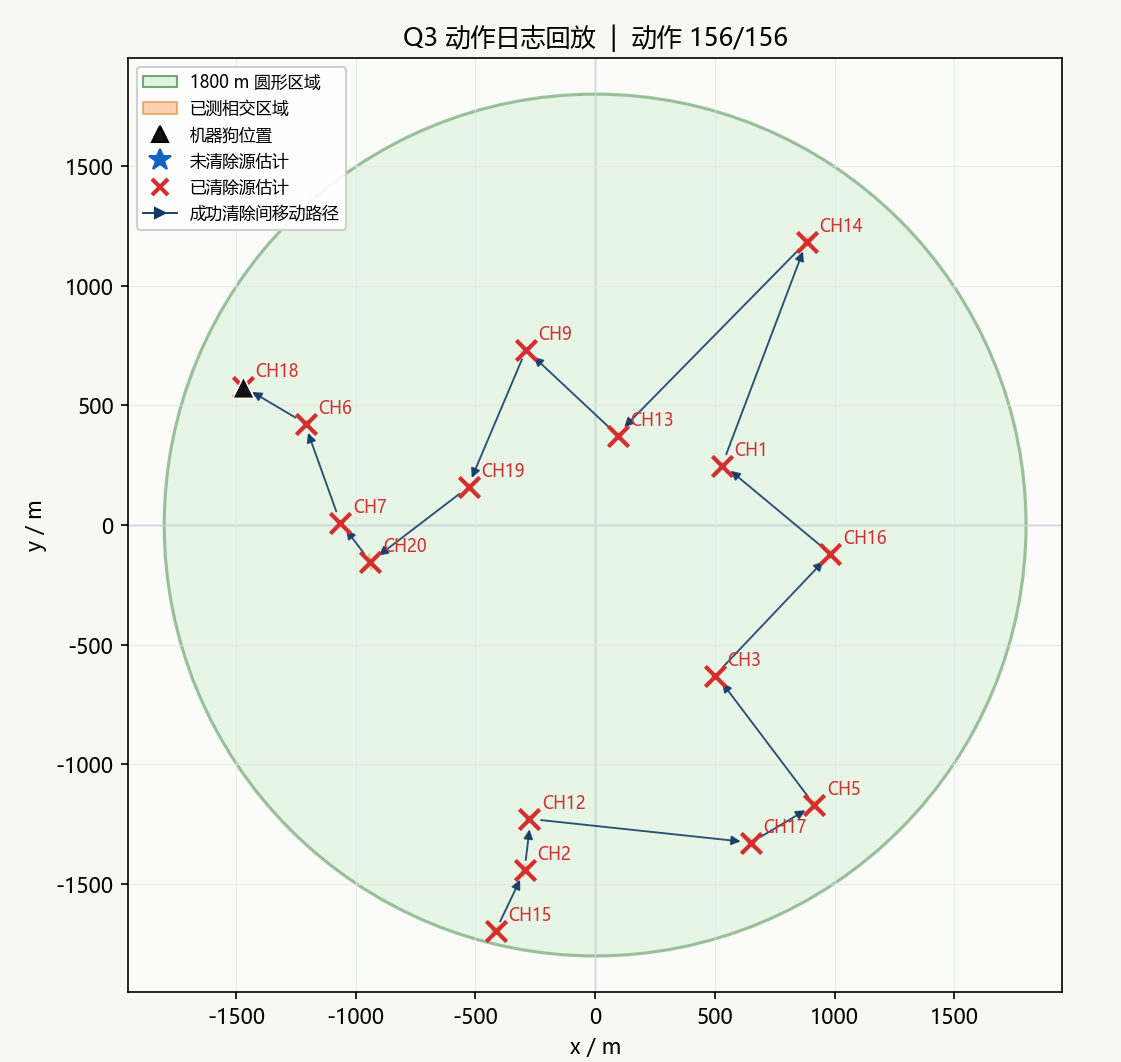
\includegraphics[width=0.72\textwidth]{figures/q3-route.png}
  \caption{问题三动作日志回放中的机器狗成功清除路线}
  \label{fig:q3-clear-route}
\end{figure}

\subsubsection{清除邻域偏移与保底覆盖}

按照开放式旅行商顺序清除已完成可靠定位的频道时，可以利用 $20\ \mathrm{m}$ 清除半径提前向下一目标移动。设当前源的最小包围圆为 $\overline B(c_j,r_j)$，下一队列中心为 $c_q$。当 $c_q\ne c_j$ 时，定义实际清除点
\begin{equation}
  y_j=c_j+(20-r_j)\frac{c_q-c_j}{\|c_q-c_j\|_2},
  \qquad r_j\leq19.9.
  \label{eq:q3-tspn-point}
\end{equation}

若当前源为最后一个源，或两中心重合，则取 $y_j=c_j$。

对任意真实源位置 $X_j\in\widehat K_j$，由三角不等式，
\begin{equation}
  \|X_j-y_j\|_2
  \leq\|X_j-c_j\|_2+\|c_j-y_j\|_2
  \leq r_j+(20-r_j)=20\ \mathrm m.
\end{equation}

因此偏移后仍能可靠清除，并沿下一目标方向前移 $20-r_j$ 米。

对尚未完成可靠定位的频道，策略先在 $c_j$ 试清除；失败后依次访问有限个保底清除点。为说明完整保底清除点构造，设 $k=\lceil r_j/20\rceil$，在中心放置一个保底清除点，并在第 $\ell$ 个同心圆上均匀放置 $6\ell$ 个保底清除点：
\begin{equation}
  q_{\ell,m}=c_j+20\ell
  \left(\cos\frac{2\pi m}{6\ell},
  \sin\frac{2\pi m}{6\ell}\right),
  \quad
  \ell=1,\ldots,k,\quad m=0,\ldots,6\ell-1.
  \label{eq:q3-probes}
\end{equation}

若某个保底清除点落在 $\widehat K_j$ 外，则将其投影到该凸多边形的最近点。完整保底清除点数量为
\begin{equation}
  N_{\mathrm{probe}}(k)=1+\sum_{\ell=1}^{k}6\ell
  =1+3k(k+1).
  \label{eq:q3-probe-count}
\end{equation}

\noindent\textbf{命题 4：}{\kaishu 式~\eqref{eq:q3-probes} 生成的不经过投影的保底清除点集合，以每个点 $20\ \mathrm{m}$ 的作用半径覆盖最小包围圆 $\overline B(c_j,r_j)$；将其中落在凸区域 $\widehat K_j$ 外的点投影到 $\widehat K_j$ 边界后，对 $\widehat K_j$ 内任意真实源位置的覆盖性质仍然成立。}

\noindent\textbf{证明：}
任取 $X\in\overline B(c_j,r_j)$。若 $\rho=\|X-c_j\|_2\leq10$，中心点即可覆盖；
否则取最近整数环号及该环上极角最近的点，则
$|\rho-20\ell|\leq10$、$|\Delta|\leq\pi/(6\ell)$。由余弦定理，
\begin{align}
  \|X-q_{\ell,m}\|_2^2
  &=(\rho-20\ell)^2+2\rho(20\ell)(1-\cos\Delta)\\
  &\leq100+\rho(20\ell)\frac{\pi^2}{36\ell^2}\\
  &\leq100+\frac{(20\ell+10)(20\ell)\pi^2}{36\ell^2}\\
  &\leq100+\frac{50\pi^2}{3}<400.
\end{align}

故存在距离小于 $20\ \mathrm m$ 的保底点。若 $q\notin\widehat K_j$，凸集投影满足
\begin{equation}
  \|X-\Pi_{\widehat K_j}(q)\|_2^2
  \leq\|X-q\|_2^2,
  \qquad X\in\widehat K_j,
\end{equation}

故投影不破坏覆盖。\hfill$\square$

每频道最多保留 $76$ 个保底点。当 $r_j\leq80\ \mathrm m$ 时完整点数至多为 $61$，覆盖保证保留；
$r_j>80\ \mathrm m$ 时队列会被截断，只能视为有限次尝试。

执行清除队列时，若当前点清除成功，则将频道加入 $\mathcal C_c$ 并转向下一队列；若失败，则删除当前队首并尝试下一个保底清除点。若所有频道最终满足
\begin{equation}
  \mathcal C_a\cup\mathcal C_c=\{1,2,\ldots,20\},
  \qquad \mathcal C_a\cap\mathcal C_c=\varnothing,
  \label{eq:q3-exit-condition}
\end{equation}

机器狗发出退出动作。在模拟器响应符合题设且保底分支满足 $r_j\leq80\ \mathrm m$ 时，
八点扫描、至多两次补充定位和有限清除队列保证策略在有限动作内完成。完整过程见
图~\ref{fig:q3-decision-tree}。

\begin{figure}[H]
  \centering
  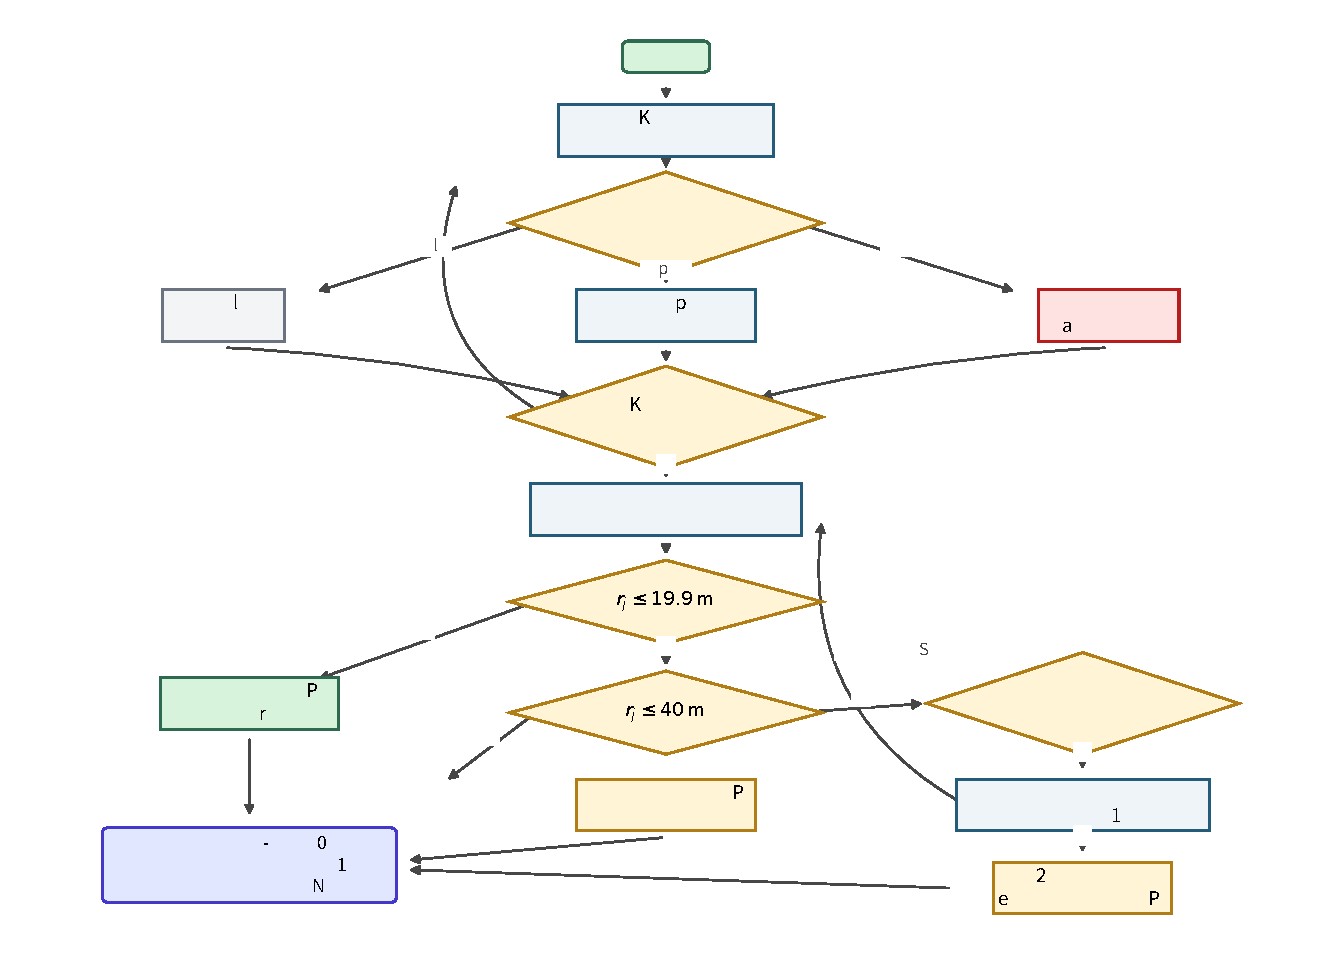
\includegraphics[width=0.98\textwidth]{figures/q3-decision-tree.pdf}
  \caption{问题三机器狗搜索、定位、路线排序与清除的决策树}
  \label{fig:q3-decision-tree}
\end{figure}

\subsection{问题四的模型建立与求解}

问题四继续使用问题三的行动时间计算、示向区域递推、最小包围圆、可靠清除点、清除邻域偏移和终止判断，本节不再重复这些结论的证明，只讨论定向干扰源带来的新增状态与决策方法。

\subsubsection{定向可见性与联合状态}

设频道 $j$ 的干扰源位置为 $x_j\in\mathcal D$，有效接收半径为 $R_j\in[1000,1500]$，类型为 $\kappa_j$。当 $\kappa_j$ 为定向时，再以 $\psi_j$ 表示最大场强方向，并记
\begin{equation}
  u(\psi_j)=
  \left(
    \cos\frac{\pi\psi_j}{180},
    \sin\frac{\pi\psi_j}{180}
  \right)^{\mathsf T}.
  \label{eq:q4-direction-vector}
\end{equation}

对联合状态 $\xi=(x,R,\psi,\kappa)$，定义检测点 $s$ 的可接收指示量

\begin{equation}
  V(\xi,s)=
  \mathbf 1_{\{\|s-x\|_2\leq R\}}
  \begin{cases}
    1, & \kappa=\text{全向},\\
    \mathbf 1_{\{u(\psi)^{\mathsf T}(s-x)\geq0\}},
       & \kappa=\text{定向}.
  \end{cases}
  \label{eq:q4-visibility}
\end{equation}

定向接收须同时满足距离与发射正面限制；无信号不能直接用于删除位置圆盘。

对每个已发现频道，除问题三已有的位置外近似 $\widehat K_j$ 外，再维护有限可能状态集合
\begin{equation}
  \Xi_j=
  \left\{\xi_\ell=(x_\ell,R_\ell,\psi_\ell,
  \kappa_\ell,w_\ell)\right\}_{\ell=1}^{L_j},
  \qquad \sum_{\ell=1}^{L_j}w_\ell=1.
  \label{eq:q4-state-set}
\end{equation}

其中位置取不超过 $12$ 个代表点，半径取 $1000$、$1250$、$1500\ \mathrm m$，定向角按
$10^\circ$ 等间隔并补充历史检测方向及其 $\pm90^\circ$ 边界。全向类和定向类初始权重各取 $0.5$，
更新后重新归一化。

可能状态须与全部历史结果相容：无信号要求 $V=0$，近距离要求 $V=1$ 且距离不超过
$5\ \mathrm m$，有效示向度还要求真实方位落在误差范围内。因此
\begin{equation}
  \Xi_j^{(m)}=
  \left\{\xi\in\Xi_j^{(m-1)}:
  \xi\text{ 与 }(s_m,y_m)\text{ 相容}\right\}.
  \label{eq:q4-state-update}
\end{equation}

有限状态利用无信号信息选点，连续位置区域仍仅按有效示向度更新，以保持凸性和保守包含。

\subsubsection{二十五个三角网驻留点的初始扫描}

问题三的八点布局只保证任意源位置附近存在一个驻留点。若该点位于定向源背面，即使距离小于 $1000\ \mathrm{m}$ 也可能收不到信号。为同时控制距离和接近方向，本文在平面上建立等边三角网。

取三角网边长 $d_4=985\ \mathrm{m}$，平移参数 $\gamma_1=\gamma_2=0.112$，令
\begin{equation}
  Q_{ij}=d_4
  \left(
    i+\gamma_1+\frac{j+\gamma_2}{2},
    \frac{\sqrt3}{2}(j+\gamma_2)
  \right),
  \qquad i,j\in\mathbb Z.
  \label{eq:q4-triangular-lattice}
\end{equation}

保留所有与 $\mathcal D$ 相交的网格三角形，其顶点并集为 $\mathcal P_4$；上述参数得到
$25$ 个驻留点和 $33$ 个三角形。

机器狗从原点按最近邻构造开放顺序，再以确定性 $2$-opt 改进；该顺序不作为最短路径结论。
驻留点、访问顺序及接收半圆见图~\ref{fig:q4-triangular-scan}。

\begin{figure}[H]
  \centering
  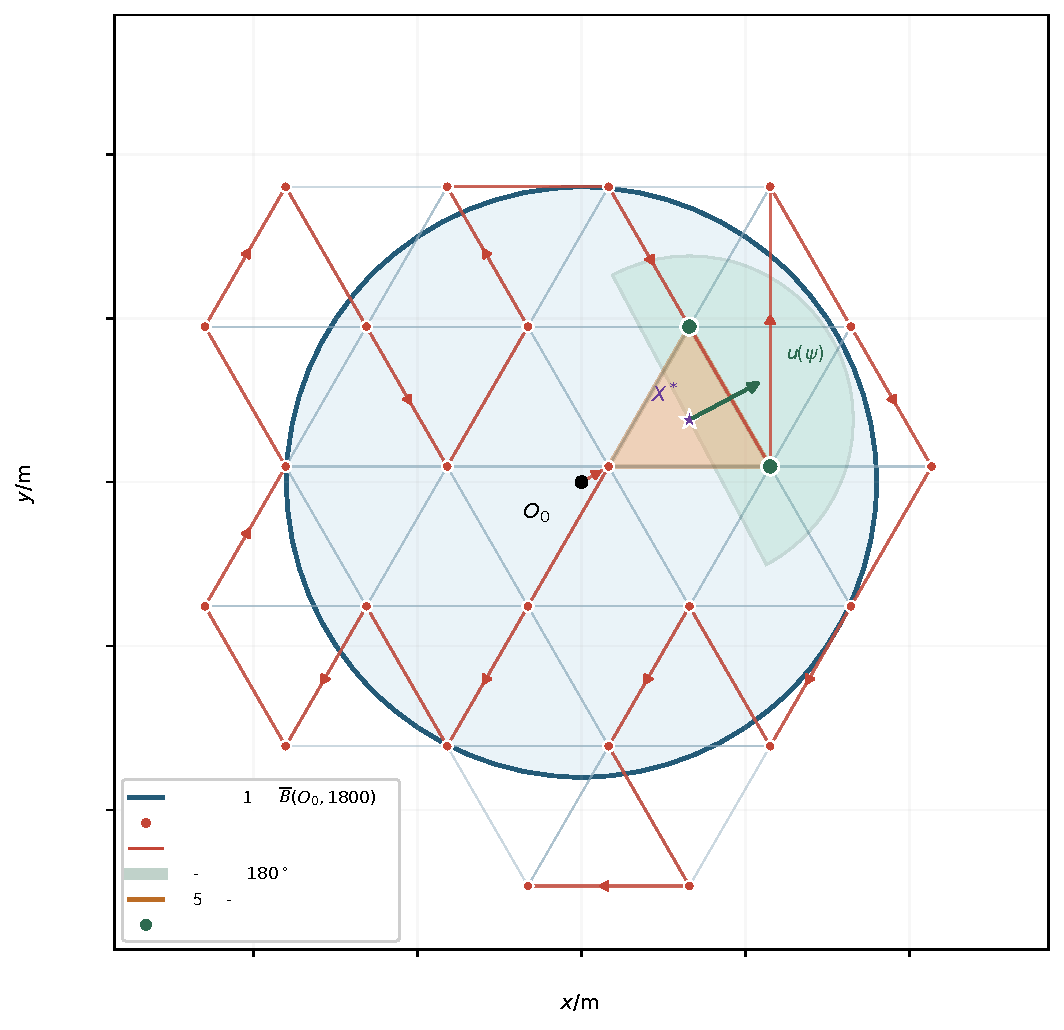
\includegraphics[width=0.83\textwidth]{figures/q4-triangular-scan.pdf}
  \caption{三角网扫描及定向覆盖：红线表示访问顺序，源 $X^*$ 的绿色接收半圆至少包含所在三角形的一个顶点}
  \label{fig:q4-triangular-scan}
\end{figure}

\noindent\textbf{命题 5：}{\kaishu 当三角网边长 $d_4\leq R_{\min}$ 时，集合 $\mathcal P_4$ 能够保证目标圆形区域内任一全向或定向干扰源至少在一个驻留点被发现。}

\noindent\textbf{证明：}
任取 $x\in\mathcal D$，存在保留的网格三角形 $T=\operatorname{conv}\{A,B,C\}$ 包含 $x$。
等边三角形直径等于边长，故
\begin{equation}
  \|A-x\|_2,\ \|B-x\|_2,\ \|C-x\|_2
  \leq d_4\leq R_{\min}.
  \label{eq:q4-triangle-distance}
\end{equation}

全向源在三个顶点均可接收。对定向源，将 $x$ 写成三顶点的凸组合；若三点均严格位于背面，则
\begin{equation}
  \begin{aligned}
    0&=u(\psi)^{\mathsf T}
    \left(\lambda_AA+\lambda_BB+\lambda_CC-x\right)\\
    &=\sum_{Q\in\{A,B,C\}}\lambda_Q u(\psi)^{\mathsf T}(Q-x)<0,
  \end{aligned}
\end{equation}

矛盾，故至少一个顶点同时满足方向与距离条件。\hfill$\square$

每个驻留点检测尚未清除的频道：近距离时原地清除，有效示向度时更新 $\widehat K_j$ 和
$\Xi_j$，无信号时仅更新 $\Xi_j$。扫描结束后，未发现频道归入无源集合。

\subsubsection{四侧探测组与局部三角网}

扫描后选择区域中心距当前位置最近的未处理频道；满足可靠条件则清除，否则构造多方向探测组。

设当前区域满足 $\widehat K_j\subseteq\overline B(c_j,r_j)$。

在中心的四个坐标轴方向设置
\begin{equation}
  \mathcal G_j^{\square}=
  \left\{
  c_j+(\rho_j,0),\ c_j+(0,\rho_j),
  c_j-(\rho_j,0),\ c_j-(0,\rho_j)
  \right\}.
  \label{eq:q4-four-sided-points}
\end{equation}

偏移量需要满足
\begin{equation}
  \sqrt2r_j<\rho_j\leq R_{\min}-r_j.
  \label{eq:q4-four-sided-condition}
\end{equation}

该区间非空要求 $r_j<R_{\min}/(1+\sqrt2)\approx414.214\ \mathrm m$；程序优先取接近 $200\ \mathrm m$ 的可行偏移量。

\noindent\textbf{命题 6：}{\kaishu 若式~\eqref{eq:q4-four-sided-condition} 成立，则对 $\widehat K_j$ 中任一可能源位置和任一发射方向，四侧探测点中至少有一个能够接收到该源信号。}

\noindent\textbf{证明：}
任取 $x\in\widehat K_j$。对任一四侧探测点 $q$，由三角不等式，
\begin{equation}
  \|q-x\|_2
  \leq\|q-c_j\|_2+\|c_j-x\|_2
  \leq\rho_j+r_j\leq R_{\min}.
  \label{eq:q4-four-distance}
\end{equation}

又由 $\|x-c_j\|_1\leq\sqrt2r_j<\rho_j$，源位于四点凸包内部；凸组合论证表明任一发射
正面至少包含一个满足距离条件的探测点。\hfill$\square$

四侧偏移不可行时，在外接矩形上铺设边长 $900\ \mathrm m$ 的局部三角网；探测组采用三种平移，
其方向覆盖理由与命题5相同。

探测组在得到有效示向度或近距离结果后结束；无信号时更新状态并选择组内剩余点。
每频道最多开始两个完整探测组。

\subsubsection{基于尾部风险的滚动选点}

利用有限联合状态，比较探测组的访问顺序及立即清除的预计时间，决定是否继续检测。

在区域外接矩形上建立边长 $27\ \mathrm m$ 的方格，其半对角线
$19.092\ \mathrm m<20\ \mathrm m$；按最近邻访问所得时间记为 $C_{\mathrm{base}}$，
再加入转向其他源的移动时间得到 $C_{\mathrm{clr}}$。实际清除仍沿用问题三的点列。

对访问顺序 $\pi$ 和状态 $\xi$ 累加行动时间；有效示向度分三种误差值预测新区域，并以
\begin{equation}
  \widehat C_{\mathrm{clr}}'
  =\max\left\{5,
  C_{\mathrm{base}}
  \left(\frac{r_j'}{r_j}\right)^2\right\}
  \label{eq:q4-clear-cost-scale}
\end{equation}

估计区域缩小后的清除时间，从而得到 $C(\pi,\xi)$。

将有限可能状态的相对权重归一化后，采用 Rockafellar 和 Uryasev 给出的等价优化形式~\cite{rockafellar2000}，以分位水平 $\alpha_R=0.9$ 的条件尾部均值评价较慢部分的完成时间：
\begin{equation}
  \mathcal R_{0.9}(\pi)
  =\min_{\eta\in\mathbb R}
  \left[
    \eta+\frac{1}{1-0.9}
    \sum_{\xi\in\Xi_j}w_\xi
    \bigl(C(\pi,\xi)-\eta\bigr)_+
  \right].
  \label{eq:q4-cvar}
\end{equation}

该指标关注耗时最长的 $10\%$ 状态。在线保留不超过 $8$ 个候选首点和 $48$ 个代表状态，记
\begin{equation}
  \pi^*=\operatorname*{arg\,min}_{\pi}\mathcal R_{0.9}(\pi).
\end{equation}

仅当
\begin{equation}
  \mathcal R_{0.9}(\pi^*)+\Delta_s<C_{\mathrm{clr}},
  \qquad \Delta_s=10\ \mathrm{s},
  \label{eq:q4-measure-or-clear}
\end{equation}

才执行 $\pi^*$ 的第一个测点，否则立即清除；每次响应后重新更新并求解，形成滚动决策。

计算上限为 $3\ \mathrm s$；状态为空、异常或超时则采用几何清除方案。有限状态只影响行动先后，
不改变清除覆盖保证。

\subsubsection{清除反馈、长尾处理与退出}

当定位半径 $r_j\leq19.9\ \mathrm{m}$ 时，直接沿用问题三的可靠清除点；当 $19.9<r_j\leq40\ \mathrm{m}$ 且尚未在中心试清除时，先在 $c_j$ 尝试一次。其余情况按式~\eqref{eq:q4-measure-or-clear} 在多方向探测与清除覆盖之间选择。

若在点 $y$ 清除失败，则由题设清除规则可知真实源位置满足 $\|x_j-y\|_2>20$。因此将有限可能状态更新为
\begin{equation}
  \Xi_j\leftarrow
  \left\{\xi\in\Xi_j:\|x_\xi-y\|_2>20\right\}.
  \label{eq:q4-failed-clear-update}
\end{equation}

清除失败后筛除有限状态并删除队首。满足剩余点数、位置和预计节省条件时可原地补测，每源至多三次；
连续失败 $8$ 次可再启动一次探测组，但不能替代完整覆盖。

多个未处理源按最近中心或清除点优先；清除成功后移入已清除集合，扫描未发现的频道移入无源集合。
满足式~\eqref{eq:q3-exit-condition} 时退出，完整过程见图~\ref{fig:q4-decision-tree}。

\begin{figure}[H]
  \centering
  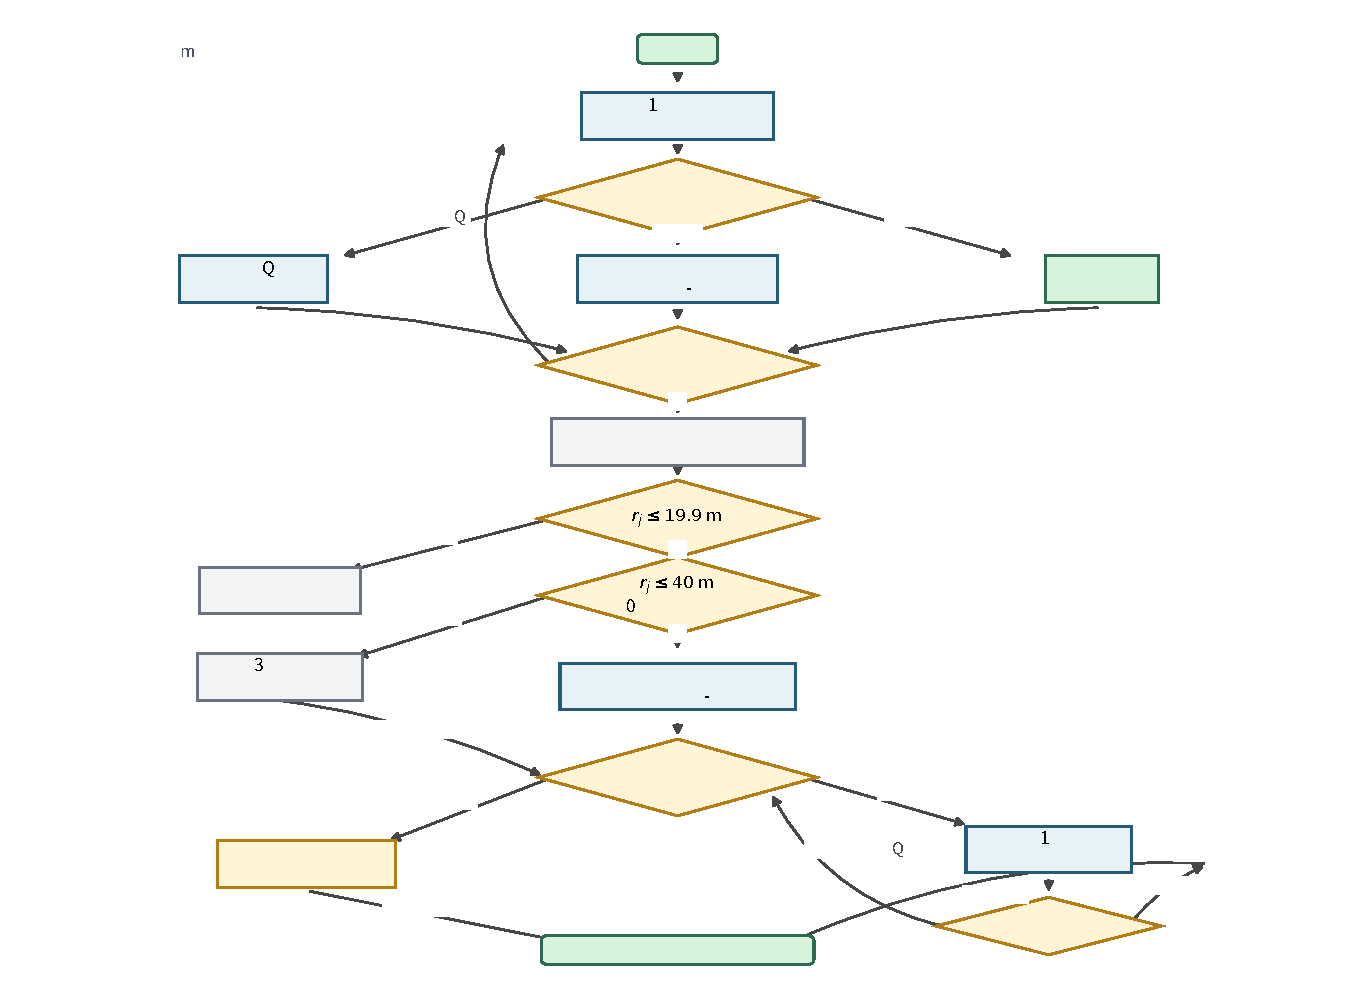
\includegraphics[width=0.98\textwidth]{figures/q4-decision-tree.pdf}
  \caption{问题四机器狗的定向扫描、联合状态更新、滚动选点与反馈清除决策树}
  \label{fig:q4-decision-tree}
\end{figure}


\section{模型检验与结果分析}

报告误差分析、敏感性分析、稳健性检验或与基准方法的比较。图表应有编号、标题、单位和必要的数据来源说明。


\section{模型评价与改进}

\subsection{模型的优点}

\begin{enumerate}
  \item \textbf{几何边界明确，关键结论可复核。}
  定位区域、保证接收域的包含关系与近似误差均有明确几何含义。

  \item \textbf{四个问题之间形成连续的决策链。}
  模型从交会定位、选点扩展到扫描、路径清除和定向源决策，前后直接复用。

  \item \textbf{理论完成条件与模拟结果相互印证。}
  两类布局和清除点列给出条件，问题三、四的50次日志清除比例均为 $100\%$。
\end{enumerate}

\subsection{模型的局限性}

\begin{enumerate}
  \item \textbf{有限离散与替代目标限制了最优性结论。}
  有限场景、Fisher 指标和有限状态只能支持当前候选集内的比较。

  \item \textbf{搜索、定位与路径规划仍采用分阶段优化。}
  补充定位、清除邻域和访问顺序未统一优化，不能证明任务总时间最短。

  \item \textbf{极端几何和长尾分支的保证具有条件。}
  近共线容差、半径超过 $80\ \mathrm m$ 的截断及有限状态使完成性结论具有条件。
\end{enumerate}

\subsection{模型的改进方向}

\begin{enumerate}
  \item \textbf{采用自适应几何精度。}
  按边界夹角和区域尺度调整外包边数，并稳健处理近共线交点。

  \item \textbf{直接围绕最终评价指标优化选点。}
  在高敏感位置增加场景，直接优化最坏定位半径和行动时间。

  \item \textbf{将定位、清除与路线进行滚动联合规划。}
  将区域收缩、清除邻域和后续访问顺序纳入有限时域模型。
\end{enumerate}


\section{结论}

逐项回答赛题提出的问题，给出可复核的核心数值、判断或建议，并保持与摘要和正文结果一致。



% 本模板整理过程使用了 AI；若后续用途变化，请据实修改花括号中的简要用途。
\CumcmAIUsed{LaTeX 模板整理与排版检查}


\begin{thebibliography}{9}
  \bibitem{toussaint1983}
  Toussaint G T.
  \newblock Solving geometric problems with the rotating calipers[C/OL]//Proceedings of IEEE MELECON'83.
  \newblock Athens, Greece: IEEE, 1983: A10.02/1--4[2026-09-11].
  \newblock \url{https://www-cgrl.cs.mcgill.ca/~godfried/research/calipers.html}.

  \bibitem{fisher1922}
  Fisher R A.
  \newblock On the mathematical foundations of theoretical statistics[J].
  \newblock Philosophical Transactions of the Royal Society of London. Series A,
  1922, 222: 309--368. DOI: \url{https://doi.org/10.1098/rsta.1922.0009}.

  \bibitem{cumcmthesis}
  LaTeX Studio.
  \newblock CUMCMThesis：全国大学生数学建模竞赛 \LaTeX{} 论文模板[CP/OL].
  \newblock 版本 2.9, 2026-08-26 [2026-09-10]. \url{https://github.com/latexstudio/CUMCMThesis}.

  % 按正文首次引用顺序继续添加文献；所有公开资料和网上资料均须在正文标注。
\end{thebibliography}

\clearpage
\begin{appendices}

\section{支撑材料文件列表}

支撑材料以文件夹“支撑材料/”为根目录。表~\ref{tab:supporting-files}
按相对于该根目录的路径列出所附材料及用途；其中正式测试日志、运行结果和
测试代码仅作目录级说明，源程序则按实际文件树逐项说明。

\begingroup
\small
\renewcommand{\arraystretch}{1.08}
\begin{longtable}{@{}>{\raggedright\arraybackslash}p{0.43\textwidth}
                        >{\raggedright\arraybackslash}p{0.52\textwidth}@{}}
  \caption{支撑材料文件列表}
  \label{tab:supporting-files}\\
  \toprule
  相对路径 & 内容与用途 \\
  \midrule
  \endfirsthead

  \multicolumn{2}{c}{表~\thetable\ （续）}\\
  \toprule
  相对路径 & 内容与用途 \\
  \midrule
  \endhead

  \midrule
  \multicolumn{2}{r}{续下页}\\
  \endfoot

  \bottomrule
  \endlastfoot

  \texttt{AI工具使用详情.pdf}
    & AI工具使用详情。 \\ 
  \path{formal_test/}
    & 正式测试日志。 \\
  \path{solution/}
    & 完整的求解程序、运行入口、测试代码与结果文件。 \\
  \path{solution/.gitignore}
    & 规定 Python 缓存、临时文件及本地生成物的忽略规则。 \\
  \path{solution/README.md}
    & 给出问题三、问题四在线测试及日志可视化的基本运行方法。 \\
  \path{solution/requirements.txt}
    & 列出运行求解程序和绘图程序所需的 Python 依赖。 \\
  \path{solution/run_drill.py}
    & 问题三、问题四连接模拟器的统一入口，负责安全确认、策略启动、逐动作日志记录及虚拟时间复算。 \\
  \path{solution/output/}
    & 离线测试和在线测试结果。 \\
  \path{solution/src/}
    & 问题一至问题四的算法实现、公共模型、运行层和模拟器通信层。 \\

  \path{solution/src/common/__init__.py}
    & 公共模块的软件包入口。 \\
  \path{solution/src/common/budget.py}
    & 实现规划过程共享的墙钟时间预算，在预算耗尽时返回当前最优结果。 \\
  \path{solution/src/common/domain.py}
    & 构造物理先验、圆形区域的保守多边形近似以及观测对应的可行域。 \\
  \path{solution/src/common/models.py}
    & 定义测向观测、机器人动作、时间分解和运行摘要等公共数据结构。 \\
  \path{solution/src/common/time_model.py}
    & 按题目规则计算移动、切换频道、测量和清除动作的虚拟时间。 \\

  \path{solution/src/legacy/environment.py}
    & 早期全向干扰源合成环境，现用于旧算法与几何行为的离线回归检查。 \\

  \path{solution/src/q1/__init__.py}
    & 汇总并导出问题一的分析与定位接口。 \\
  \path{solution/src/q1/API.md}
    & 说明问题一输入数据、返回字段及模块接口约定。 \\
  \path{solution/src/q1/bearing_plot.py}
    & 绘制检测点、示向线、误差扇区和定位区域。 \\
  \path{solution/src/q1/cli.py}
    & 问题一命令行入口，读取测向数据并输出定位分析及图形。 \\
  \path{solution/src/q1/geometry.py}
    & 实现测向扇区半平面、凸多边形求交、直径和最小包围圆等核心几何算法。 \\
  \path{solution/src/q1/README.md}
    & 说明问题一的算法流程以及各算法步骤与代码文件的对应关系。 \\

  \path{solution/src/q2/__init__.py}
    & 汇总并导出问题二的候选域构造、连续优化和测点规划接口。 \\
  \path{solution/src/q2/candidates.py}
    & 构造保证接收域、可能接收域及确定性的候选检测点集合。 \\
  \path{solution/src/q2/cli.py}
    & 问题二命令行入口，执行第二检测点规划并输出结果文件。 \\
  \path{solution/src/q2/continuous_diameter.py}
    & 以最坏情形后验包围直径为目标进行连续测点搜索，供替代目标实验使用。 \\
  \path{solution/src/q2/continuous_fim.py}
    & 在保证接收域内执行基于 Fisher 信息矩阵替代指标的连续测点优化。 \\
  \path{solution/src/q2/near_optimal.py}
    & 根据局部采样结果构造问题二的近优测点区域。 \\
  \path{solution/src/q2/planner.py}
    & 组织离散候选评分、连续优化、Pareto 筛选和最终第二测点推荐。 \\
  \path{solution/src/q2/plot.py}
    & 绘制候选区域、离散与连续方案、近优域及 Pareto 对比结果。 \\

  \path{solution/src/q3/__init__.py}
    & 问题三策略模块的软件包入口。 \\
  \path{solution/src/q3/batch_policy.py}
    & 实现当前问题三批量定位、Held--Karp 开放路径排序及分批清除策略。 \\
  \path{solution/src/q3/cli.py}
    & 问题三离线演示入口，不连接正式模拟器。 \\
  \path{solution/src/q3/coverage.py}
    & 构造全场扫描布局、覆盖检验和有限清除探针序列。 \\
  \path{solution/src/q3/minimax_leg.py}
    & 实现按最坏后验半径选择补充测量位置的极小极大实验方案。 \\
  \path{solution/src/q3/policy.py}
    & 定义全向干扰源扫描、定位、清除和退出的基础状态机。 \\
  \path{solution/src/q3/refine_selector.py}
    & 实现兼顾绕行成本和预测定位收缩效果的补充测量位置实验方案。 \\

  \path{solution/src/q4/__init__.py}
    & 问题四定向干扰源扩展模块的软件包入口。 \\
  \path{solution/src/q4/belief.py}
    & 根据位置、接收半径和发射方向的有限场景构造联合信念，用于动作排序。 \\
  \path{solution/src/q4/cli.py}
    & 问题四离线演示入口，不连接正式模拟器。 \\
  \path{solution/src/q4/directional.py}
    & 构造定向源发现扫描网、复核探测点并判定发射方向可见性。 \\
  \path{solution/src/q4/policy.py}
    & 实现问题四混合全向、定向干扰源的扫描、复核、定位和清除策略。 \\
  \path{solution/src/q4/rolling.py}
    & 以有限场景风险和后续代价评估定向探测、直接清除及保底清除动作。 \\

  \path{solution/src/runtime/__init__.py}
    & 与具体模拟器无关的运行模块入口。 \\
  \path{solution/src/runtime/runner.py}
    & 按动作上限顺序驱动策略与离线客户端，并汇总一轮运行结果。 \\

  \path{solution/src/sim/__init__.py}
    & 汇总并导出模拟器通信、协议校验、离线替身和现场运行接口。 \\
  \path{solution/src/sim/cli.py}
    & 人工准备好模拟器后的现场命令行入口，包含联通检查和完整策略模式。 \\
  \path{solution/src/sim/client.py}
    & 实现仅访问本机回环地址的同步 HTTP 客户端及安全重试和幂等控制。 \\
  \path{solution/src/sim/errors.py}
    & 定义传输、HTTP、协议、业务拒绝、并发和幂等冲突等异常类型。 \\
  \path{solution/src/sim/fake.py}
    & 提供与正式客户端具有相同执行接口的确定性离线模拟器。 \\
  \path{solution/src/sim/live_runner.py}
    & 在动作上限和退出安全余量约束下运行在线策略，并持续写入逐动作日志。 \\
  \path{solution/src/sim/protocol.py}
    & 校验并编解码题目附件规定的模拟器 HTTP 与 JSON 请求、响应。 \\
  \path{solution/src/sim/smoke.py}
    & 实现进入、单次测量和退出组成的最小联通检查策略。 \\

  \path{solution/src/simlite/__init__.py}
    & 实现无 HTTP 层的轻量离线模拟器及微秒级虚拟时间累计。 \\
  \path{solution/src/simlite/paired.py}
    & 对同一随机案例池中的两种策略进行成对比较并生成晋级判定指标。 \\
  \path{solution/src/simlite/replay.py}
    & 批量回放策略，统计扫描、定位和清除时间并复核虚拟时间账目。 \\

  \path{solution/src/tools/__init__.py}
    & 辅助分析与可视化工具的软件包入口。 \\
  \path{solution/src/tools/log_visualize/}
    & 日志可视化工具。 \\

  \path{solution/tests/}
    & 测试用代码。 \\
\end{longtable}
\endgroup

\section{源程序}

本附录列出问题一至问题四正式求解程序及模拟器接口运行链路的完整
Python 源代码。文件名均以支撑材料文件夹“支撑材料/”为根目录；
代码内容直接从相应支撑材料文件载入。离线测试、旧版实现及日志分析
工具不在本附录中重复列出。

问题三和问题四的在线测试代码如下：
\begin{lstlisting}
  # Q3在线测试
  python run_drill.py --problem 3 --mode policy --robot-id "参赛队号" --confirm-ready --confirm-policy --max-actions 8000
  # Q4在线测试
  python run_drill.py --problem 4 --robot-id "参赛队号" --confirm-ready --confirm-policy
\end{lstlisting}

\begingroup
\lstset{
  language=Python,
  basicstyle=\fontspec{DejaVu Sans Mono}\scriptsize,
  numbers=left,
  numberstyle=\tiny\color{gray},
  numbersep=6pt,
  frame=single,
  breaklines=true,
  breakatwhitespace=false,
  columns=fullflexible,
  keepspaces=true,
  showstringspaces=false,
  tabsize=4,
  literate=
    {≤}{{$\leq$}}1
    {≥}{{$\geq$}}1
    {∈}{{$\in$}}1
    {⊇}{{$\supseteq$}}1
    {⊆}{{$\subseteq$}}1
    {∩}{{$\cap$}}1
    {π}{{$\pi$}}1
    {ρ}{{$\rho$}}1
    {θ}{{$\theta$}}1
}

\subsection{公共模型与时间预算}

\subsubsection*{\path{solution/src/common/__init__.py}}
\lstinputlisting{../支撑材料/solution/src/common/__init__.py}

\subsubsection*{\path{solution/src/common/budget.py}}
\lstinputlisting{../支撑材料/solution/src/common/budget.py}

\subsubsection*{\path{solution/src/common/domain.py}}
\lstinputlisting{../支撑材料/solution/src/common/domain.py}

\subsubsection*{\path{solution/src/common/models.py}}
\lstinputlisting{../支撑材料/solution/src/common/models.py}

\subsubsection*{\path{solution/src/common/time_model.py}}
\lstinputlisting{../支撑材料/solution/src/common/time_model.py}

\subsection{问题一源程序}

\subsubsection*{\path{solution/src/q1/__init__.py}}
\lstinputlisting{../支撑材料/solution/src/q1/__init__.py}

\subsubsection*{\path{solution/src/q1/bearing_plot.py}}
\lstinputlisting{../支撑材料/solution/src/q1/bearing_plot.py}

\subsubsection*{\path{solution/src/q1/cli.py}}
\lstinputlisting{../支撑材料/solution/src/q1/cli.py}

\subsubsection*{\path{solution/src/q1/geometry.py}}
\lstinputlisting{../支撑材料/solution/src/q1/geometry.py}

\subsection{问题二源程序}

\subsubsection*{\path{solution/src/q2/__init__.py}}
\lstinputlisting{../支撑材料/solution/src/q2/__init__.py}

\subsubsection*{\path{solution/src/q2/candidates.py}}
\lstinputlisting{../支撑材料/solution/src/q2/candidates.py}

\subsubsection*{\path{solution/src/q2/cli.py}}
\lstinputlisting{../支撑材料/solution/src/q2/cli.py}

\subsubsection*{\path{solution/src/q2/continuous_diameter.py}}
\lstinputlisting{../支撑材料/solution/src/q2/continuous_diameter.py}

\subsubsection*{\path{solution/src/q2/continuous_fim.py}}
\lstinputlisting{../支撑材料/solution/src/q2/continuous_fim.py}

\subsubsection*{\path{solution/src/q2/near_optimal.py}}
\lstinputlisting{../支撑材料/solution/src/q2/near_optimal.py}

\subsubsection*{\path{solution/src/q2/planner.py}}
\lstinputlisting{../支撑材料/solution/src/q2/planner.py}

\subsubsection*{\path{solution/src/q2/plot.py}}
\lstinputlisting{../支撑材料/solution/src/q2/plot.py}

\subsection{问题三源程序}

\subsubsection*{\path{solution/src/q3/__init__.py}}
\lstinputlisting{../支撑材料/solution/src/q3/__init__.py}

\subsubsection*{\path{solution/src/q3/batch_policy.py}}
\lstinputlisting{../支撑材料/solution/src/q3/batch_policy.py}

\subsubsection*{\path{solution/src/q3/cli.py}}
\lstinputlisting{../支撑材料/solution/src/q3/cli.py}

\subsubsection*{\path{solution/src/q3/coverage.py}}
\lstinputlisting{../支撑材料/solution/src/q3/coverage.py}

\subsubsection*{\path{solution/src/q3/minimax_leg.py}}
\lstinputlisting{../支撑材料/solution/src/q3/minimax_leg.py}

\subsubsection*{\path{solution/src/q3/policy.py}}
\lstinputlisting{../支撑材料/solution/src/q3/policy.py}

\subsubsection*{\path{solution/src/q3/refine_selector.py}}
\lstinputlisting{../支撑材料/solution/src/q3/refine_selector.py}

\subsection{问题四源程序}

\subsubsection*{\path{solution/src/q4/__init__.py}}
\lstinputlisting{../支撑材料/solution/src/q4/__init__.py}

\subsubsection*{\path{solution/src/q4/belief.py}}
\lstinputlisting{../支撑材料/solution/src/q4/belief.py}

\subsubsection*{\path{solution/src/q4/cli.py}}
\lstinputlisting{../支撑材料/solution/src/q4/cli.py}

\subsubsection*{\path{solution/src/q4/directional.py}}
\lstinputlisting{../支撑材料/solution/src/q4/directional.py}

\subsubsection*{\path{solution/src/q4/policy.py}}
\lstinputlisting{../支撑材料/solution/src/q4/policy.py}

\subsubsection*{\path{solution/src/q4/rolling.py}}
\lstinputlisting{../支撑材料/solution/src/q4/rolling.py}

\subsection{正式运行层}

\subsubsection*{\path{solution/src/runtime/__init__.py}}
\lstinputlisting{../支撑材料/solution/src/runtime/__init__.py}

\subsubsection*{\path{solution/src/runtime/runner.py}}
\lstinputlisting{../支撑材料/solution/src/runtime/runner.py}

\subsection{模拟器接口}

\subsubsection*{\path{solution/src/sim/__init__.py}}
\lstinputlisting{../支撑材料/solution/src/sim/__init__.py}

\subsubsection*{\path{solution/src/sim/cli.py}}
\lstinputlisting{../支撑材料/solution/src/sim/cli.py}

\subsubsection*{\path{solution/src/sim/client.py}}
\lstinputlisting{../支撑材料/solution/src/sim/client.py}

\subsubsection*{\path{solution/src/sim/errors.py}}
\lstinputlisting{../支撑材料/solution/src/sim/errors.py}

\subsubsection*{\path{solution/src/sim/fake.py}}
\lstinputlisting{../支撑材料/solution/src/sim/fake.py}

\subsubsection*{\path{solution/src/sim/live_runner.py}}
\lstinputlisting{../支撑材料/solution/src/sim/live_runner.py}

\subsubsection*{\path{solution/src/sim/protocol.py}}
\lstinputlisting{../支撑材料/solution/src/sim/protocol.py}

\subsubsection*{\path{solution/src/sim/smoke.py}}
\lstinputlisting{../支撑材料/solution/src/sim/smoke.py}

\endgroup


\end{appendices}

\end{document}
